%%%%%%%%%%%%%%%%%%%%%%%%%%%%%%%%%%%%%%%%%%%%%%%%%%%%%%%%%%%%%%%%%%%%%%%%%%%%%%%
% Frame for Bachelor or Master Thesis at FAU/i1
% Topic: [Title of thesis]
% Copyright (C) 2012  [Author]
% based on original work by Johannes Goetzfried, used with permission
%%%%%%%%%%%%%%%%%%%%%%%%%%%%%%%%%%%%%%%%%%%%%%%%%%%%%%%%%%%%%%%%%%%%%%%%%%%%%%%

%%%%%%%%%%%%%%%%%%%%%%%%%%%%%%%%%%%%%%%%%%%%%%%%%%%%%%%%%%%%%%%%%%%%%%%%%%%%%%%
%
% Header
% 
%%%%%%%%%%%%%%%%%%%%%%%%%%%%%%%%%%%%%%%%%%%%%%%%%%%%%%%%%%%%%%%%%%%%%%%%%%%%%%%

% Font size and paper
\documentclass[10pt,twoside,a4paper,bibliography=totoc]{scrbook}

% A few commands
\newcommand{\term}[1]{\textit{#1}}
\newcommand{\code}[1]{\texttt{#1}}
\newcommand{\echoName}[1]{Christoph Neubauer}
\newcommand{\echoOther}[1]{Tobias Krau{\ss}}
\newcommand{\echoTitle}[1]{Design and Implementation of a fault-tolerant form processing application using machine learning}

\newcommand{\todo}[1]{{\color{magenta} [TODO: #1]}}

\newcommand{\anatoli}[1]{{\color{Maroon} [Anatoli: #1]}}

% Margin
\usepackage{setspace}
\usepackage{anysize}
\marginsize{3cm}{3cm}{2cm}{2cm}

% Font, Encoding
\usepackage[T1]{fontenc}
\usepackage[utf8]{inputenc}
\usepackage{times}

% Fancy header and footer
\usepackage{fancyhdr}

% Graphics
\usepackage{graphicx}
\usepackage{float}
\graphicspath{{images/}}
\usepackage{svg}

% Math stuff
\usepackage{amsmath}
\usepackage{amssymb}
\usepackage{nicefrac}
\usepackage{tabularx}

% Code listings
\usepackage{listings}
\lstset{basicstyle=\footnotesize\ttfamily}

% Links within pdf file
\usepackage{hyperref}
\hypersetup{
	colorlinks=true,
	linkcolor=black,
	citecolor=black,
	filecolor=black,
	urlcolor=black,
	breaklinks=true,
	bookmarksnumbered=true,
	pdfstartpage={1},
        % adapt following lines if you want these items to show in pdf
        % otherwise remove
	pdftitle={\echoTitle \\},
	pdfsubject={Master Thesis},
	pdfauthor={\echoName \\}
}

% Figure captions
\usepackage{caption}
\captionsetup{font=small,labelfont=bf}

% for sample text, can be removed in production version
\usepackage{blindtext}

% Fancy toc title
\renewcommand{\contentsname}{CONTENTS}

% Fancy chapter page
\makeatletter
\def\@makechapterhead#1{
  \vspace*{100\p@}
  {\parindent \z@ 
    {\raggedleft
      \fontsize{15ex}{15ex}
      \textsf\thechapter\par\nobreak}
    \par\nobreak
    \interlinepenalty\@M
    {\raggedright \Huge \textsf{\textsc{#1}}}
    \par\nobreak
    \leavevmode \leaders \hrule height 0.65ex \hfill \kern \z@
    \par\nobreak
    \vskip 100\p@
  }
}

% No headers on empty pages before new chapter
\makeatletter
\def\cleardoublepage{\clearpage\if@twoside \ifodd\c@page\else
  \hbox{}
  \thispagestyle{plain}
  \newpage
  \if@twocolumn\hbox{}\newpage\fi\fi\fi}
\makeatother \clearpage{\pagestyle{plain}\cleardoublepage}

% Fancy header / footer for chapter pages
\fancypagestyle{plain}{
	\fancyhf{}
	\renewcommand{\headrulewidth}{0pt}
	\fancyfoot[LE,RO]{\thepage}
}

% Fancy header / footer for normal pages
\pagestyle{fancy}
\fancyhf{}
\fancyfoot[LE,RO]{\thepage}
\fancyhead[LO]{\leftmark}
\fancyhead[RE]{\rightmark}

% No indent for paragraphs
\setlength{\parskip}{1.3ex plus 0.2ex minus 0.2ex}
\setlength{\parindent}{0pt}

% Fancy bibliography, see http://merkel.zoneo.net/Latex/natbib.php
\usepackage[square,comma,numbers,sort&compress]{natbib}


\begin{document}

% Alphabetic page numbers
\pagenumbering{alph}

%%%%%%%%%%%%%%%%%%%%%%%%%%%%%%%%%%%%%%%%%%%%%%%%%%%%%%%%%%%%%%%%%%%%%%%%%%%%%%%
%
% Title
%
%%%%%%%%%%%%%%%%%%%%%%%%%%%%%%%%%%%%%%%%%%%%%%%%%%%%%%%%%%%%%%%%%%%%%%%%%%%%%%%

\begin{titlepage}

\titlehead{
	\centering
	\begin{tabular}[ht]{lcr}
		\parbox{3cm}{
			\centering
			
\includegraphics[width=2.5cm]{images/ch1/fau-logo.png}
		} &
		\parbox{5cm}{
			\centering
			Lehrstuhl für Informatik 5 \\
			Friedrich-Alexander-Universität \\
			Erlangen-Nürnberg \\
		} &
		\parbox{3cm}{
			\centering
			
\includegraphics[width=2.5cm]{images/ch1/i5-logo.png}
		}
	\end{tabular}
	\vspace{4em}
}

\subject{
	MASTER THESIS
}

% you should also adapt entries for name and title in 00-0-header.tex
% in the pdf tags (if you want)
\title{
  Design and Implementation of a fault-tolerant form processing application using machine learning
}

\author{
	\vspace{4em}
	Christoph Neubauer
}

\date{
	Erlangen, \today
}

\publishers{
	\begin{tabular}{lcl}
		Examiner:  && Prof. Dr.-Ing. habil. Andreas Maier \\
		First Advisor:   && PD Dr.-Ing. habil. Peter Wilke \\
		Second Advisor: && Prof. Dr. Luiz Eduardo S. Oliveira
	\end{tabular}
}

\maketitle
\end{titlepage}


% Roman page numbers
\pagenumbering{roman}

% Pre content
%%%%%%%%%%%%%%%%%%%%%%%%%%%%%%%%%%%%%%%%%%%%%%%%%%%%%%%%%%%%%%%%%%%%%%%%%%%%%%%
%
% Declaration 
%
%%%%%%%%%%%%%%%%%%%%%%%%%%%%%%%%%%%%%%%%%%%%%%%%%%%%%%%%%%%%%%%%%%%%%%%%%%%%%%%


% Pseudo chapter
\chapter*{\ }


\vspace*{\fill}


% Header
\begin{Large}
	\textbf{Eidesstattliche Erklärung / Statutory Declaration}
\end{Large}
\vspace{1.5em}


\noindent\hrule

% German
Hiermit versichere ich eidesstattlich, dass die vorliegende Arbeit von mir
selbständig, ohne Hilfe Dritter und ausschließlich unter Verwendung der
angegebenen Quellen angefertigt wurde. Alle Stellen, die wörtlich oder
sinngemäß aus den Quellen entnommen sind, habe ich als solche kennt\-lich
gemacht. Die Arbeit wurde bisher in gleicher oder ähnlicher Form keiner anderen
Prüfungsbehörde vorgelegt. 
\vspace{1.5em}


% English
I hereby declare formally that I have developed and written the enclosed thesis
entirely by myself and have not used sources or means without declaration in
the text. Any thoughts or quotations which were inferred from the sources are
marked as such. This thesis was not submitted in the same or a substantially
similar version to any other authority to achieve an academic grading. 

\noindent\hrule

\vspace{2em}

% remove the following text if it doesn't seem appropriate

Der Friedrich-Alexander-Universität, vertreten durch den Lehrstuhl
für Informatik 1, wird für Zwecke der Forschung und Lehre ein
einfaches, kostenloses, zeitlich und örtlich unbeschränktes
Nutzungsrecht an den Arbeitsergebnissen der Arbeit einschließlich
etwaiger Schutz- und Urheberrechte eingeräumt.


\vspace{2em}

% Sign
Erlangen, \today
\begin{flushright}
	\underline{\ \ \ \ \ \ \ \ \ \ \ \ \ \ \ \ \ \ \ \ \ \ \ \ \ 
		\ \ \ \ \ \ \ \ \ \ \ \ \ \ \ \ \ \ \ \ \ \ \ \ \ \ \ \ \ 
	} \\
	\small{\echoName\\}
\end{flushright}

%%%%%%%%%%%%%%%%%%%%%%%%%%%%%%%%%%%%%%%%%%%%%%%%%%%%%%%%%%%%%%%%%%%%%%%%%%%%%%%
%
% Abstract
% 
%%%%%%%%%%%%%%%%%%%%%%%%%%%%%%%%%%%%%%%%%%%%%%%%%%%%%%%%%%%%%%%%%%%%%%%%%%%%%%%

% Pseudo chapter
\chapter*{\ }

\vspace{2em}
\begin{center}
	\begin{large}
		\textbf{Abstract}
	\end{large}
\end{center}
\vspace{0.75em}
Virtualization still poses one the hardest obfuscation techniques known to reverse engineers. Not unlike software packers, virtualization obfuscators hamper static analysis by changing the execution flow drastically and yet, contrary to software packers the original binary code is not part of the final obfuscated virtualization routine and as such cannot be recovered mid execution. But despite the fact, that virtualization obfuscators create a protective layer that hampers static and dynamic analysis alike, research in the field of deobfuscation of virtualized binaries progressed rather slowly in the last decade. \\
This thesis developed a novel technique for an automated approach to deobfuscation of virtualized binaries by using a combination of dynamic analysis and pattern recognition. The resulting analysis capabilities were also implemented as a proof-of-concept prototype called 'VMAttack' and evaluated using test cases obfuscated with VMProtect.\\
The dynamic capabilities of VMAttack are further extended by \echoOther{}'s static analysis techniques developed in \cite{Krau:Thesis2016}. This creates a highly flexible analysis tool which supports not only dynamic but also static analysis and provides an easy to use interface for automation to combine all analysis capabilities into a more fault tolerant result. The idea was met with approval from the reversing community, even winning first place in the IDA Plug-in Contest 2016.\\
\newline

\begin{center}
	\begin{large}
		\textbf{Zusammenfassung}
	\end{large}
\end{center}
\vspace{0.75em}
Virtualisierung ist heute nach wie vor eine der am schwersten zu knackenden Obfuskierungstechnicken. Aehnlich wie Softwarepacker wird statische Analyse erschwert indem der Kontrollfluss drastisch geaendert wird. Im Gegensatz zu Softwarepackern gibt es jedoch keinen Zeitpunkt waehrend der Ausfuehrung, in dem die urspruengliche Binaerdatei wieder hergestellt wird, da sie nicht Teil der virtualisierten Version ist. Trotz dieser offensichtlichen Herausforderungen hielt sich Forschung zur Deobfuskierung von virtualisierten Binaerdateien im letzten Jahrzehnt zurueck, verglichen mit anderen Bereichen.\\
In dieser Thesis wurde eine neue Herangehensweise entwickelt fuer einen automatisierte Deobfuskierung von virtualisierten Binaerdateien. Hierfuer werden Technicken aus der dynamischen Analyse und der Mustererkennung kombiniert. Die sich hieraus ergebenden Analysen wurden als Proof-of-Concept Prototyp 'VMAttack' implementiert und mit Testfaellen eveluiert, welche durch VMProtect obfuskiert wurden.\\
Die dynamischen Analysearten von VMAttack werden durch \echoOther{}s statische Analysen ergaenzt, welche von Ihm in \cite{Krau:Thesis2016} entwickelt wurden. Damit entsteht ein hoechst flexibles Analysewerkzeug, welches dynamische und statische Analysen unterstuetzt und eine einfach benutzbare Schnittstelle fuer Automatisierung dieser Analysen bietet. Die Idee wurde wurde sehr unterstuetzt von Reverse Engineering Gemeinschaft und hat sogar den ersten Platz beim IDA Plugin Contest 2016 belegt.




% Table of Contents
\listoftables
\listoffigures
\begin{onehalfspacing}
\tableofcontents
\end{onehalfspacing}
\cleardoublepage

% Arabic page numbers
\pagenumbering{arabic}


% Actual content, can be split up into multiple files or kept in
% one big file
\fancyhead[RE]{\leftmark}
%%%%%%%%%%%%%%%%%%%%%%%%%%%%%%%%%%%%%%%%%%%%%%%%%%%%%%%%%%%%%%%%%%%%%%%%%%%%%%%
%
% Introduction
% 
%%%%%%%%%%%%%%%%%%%%%%%%%%%%%%%%%%%%%%%%%%%%%%%%%%%%%%%%%%%%%%%%%%%%%%%%%%%%%%%


\chapter{Introduction}
\label{sec1:intro}
This thesis developed a Framework for automated and manual analysis of obfuscated binaries via a virtualization obfuscator. 
Since part of the original binary is only present in the obfuscated version in form of interpretable byte code, the first main objective of a reverse engineering analysis is the interpretation of said byte code. 
To assist a reverse engineer, analysis techniques need to be developed that counteract virtualization as obfuscation measure specifically.\\ 
The main focus of this thesis was the development and prototypic implementation of dynamic analysis capabilities and additionally an automation of the analysis process as far as possible. 
This ultimately resulted in the implementation of the IDA Pro plug-in 'VMAttack', which builds upon the static virtualization analysis of \echoOther{} and combines it with new dynamic analysis techniques and dynamic optimization techniques. 
Additionally an automation system is proposed, which allows a completely automated analysis to take place while still leaving the reverse engineer in control which analysis features to are deemed important. This kind of automation not only reduces the inhibition threshold for new users but also allows for an overall more fault tolerant result. 
To automate the process even further, using IDA's batch execution mode it is even possible to run a predefined analysis combination on several samples in succession. \\
As a result the plug-ins capabilities were even recognized by Hex Rays in their annual IDA  Pro plug-in contest, where VMAttack made second place in 2016!\\


\section{Motivation}
\label{sec1:motiv}
Obfuscation increases the time a reverse engineer needs to get to unintended information. But unintended for whom? 
If software crackers use reverse engineering to recover a license key verification algorithm we consider the use of obfuscation to increase the time span to recovery of the key as far as possible.
For this very reason new obfuscation techniques are researched and are used to increase the security measures of our software.
However, obfuscation is merely a tool, a routine that can be used by both, legal and illegal entities alike. 
The same crackers despairing at an obfuscation measure might use it the next day to obfuscate a malware routine.
This is the very livelihood of deobfuscation research. By definition deobfuscation research starts only after an obfuscation technique has been `discovered' and as such has a time disadvantage where the obfuscation technique can roam free without a structured approach at deobfuscation.
One such technique is virtualization.
Contrary to simpler obfuscation techniques where deobfuscation approaches are developed soon after publication, virtualization obfuscators can be found in the wild for over a decade and are still quite successful at obfuscating what shall not be found out.
And although research is already being done on the topic of virtualization obfuscators \cite{Rolles:2009:UVO:1855876.1855877, Coogan:2011:DVS:2046707.2046739, DBLP:conf/sp/YadegariJWD15} a common approach recognized to be effective at large is still missing. The situation is aggravated further by the heavy imbalance of automation possibilities. While methods for automating the obfuscation process exist and are available commercially\cite{vm_prot, code_virt, themida} or even as freeware\cite{vm_prot}, the same can not be said for their counterpart\cite{Rolles:2009:UVO:1855876.1855877, DBLP:conf/sp/YadegariJWD15}. 
This results in more and more malware authors using additional heavy duty obfuscation to impede the reversing process of their binaries. 

In its own right, the virtualization-obfuscation technique seems particularly tough by any measure. Hereby the original program's logic is embedded within the byte code for a custom virtual machine (VM) interpreter\cite{Coogan:2011:DVS:2046707.2046739}. It is important to understand at this point that the VM can be randomized and the binary automatically repackaged with a different VM at any time, e.g. with the release of a new version\cite{DBLP:conf/sp/SharifLGL09}. Doing so would not only increase the reverse engineers efforts for deobfuscation but also defeat some conventional malware detection mechanisms employed by anti virus providers. 

On the other hand the reverse engineer when facing virtualization-obfuscated binaries has to first reverse engineer the VM interpreter, then use this information to work out individual byte code instructions and finally, recover the logic embedded in the byte code program\cite{Coogan:2011:DVS:2046707.2046739}. Even worse, the obfuscator has complete freedom to choose the semantics of the byte code instructions, and entities such as virtual registers and memory addresses can be independent from the underlying real machine\cite{DBLP:conf/sp/SharifLGL09}. This would mean that even if the reverse engineer is facing an already known binary repackaged with a different obfuscator, the time consuming task of reversing the VM interpreter has to be repeated. Since this task is still a manual process we can observe a disparity between the automated obfuscation and the manual deobfuscation concerning the expected duration of both.

Previous semester \echoOther{} already started the endeavors to create a framework for the Interactive Disassembler (IDA) which would enable the automation of the process of reversing the virtual machine and the virtual code\cite{Krau:Thesis2016}. This framework was improved to a fully fledged IDA plug-in offering the previously developed static deobfuscation analysis and additionally providing dynamic analysis techniques, an increased level of automation and an interface for the reverse engineer to shape the parameters of static and dynamic analysis at will.

At present the framework consists of an automated static analysis module which enables the reverse engineer to automate the static analysis of the VM interpreter and virtual byte code. The results of this analysis are presented in an intermediate representation (IR) language which also was developed by \echoOther{}\cite{Krau:Thesis2016}. If this framework was to be extended to contain a more diverse selection of analysis functionalities, it would represent a great leap towards balancing out the disparities between the already automated virtualization-obfuscation and the mostly manual deobfuscation of virtualization-obfuscated binaries.


\section{Task}
\label{sec1:task}
The task of this master thesis is to evaluate different electronic invoice formats. 
An application shall be designed and implemented that processes invoice forms and is capable of storing them in the invoice format that suits the most.
The application should use machine learning in order to improve processing accuracy over time.
Nevertheless, errors during the scan process should be handled by the application itself.

The output of this application should be conform with the definition of the electronic invoice format that has been decided in beforehand.



\section{Related Work}
\label{sec1:relwork}
VMAttack is a virtual-packed binary analysis and deobfuscation framework, with support for static and dynamic analysis in addition to automation capabilities. As other attempts at devirtualization have been made as well, this section will distinguish VMAttack from other approaches. As the focus of this thesis lies primarily on dynamic analysis and automation this will be used as differentiation criteria. A similiar differentiation analysis was provided for the static analysis of VMAttack in \cite{Krau:Thesis2016}. Since the static or dynamic approaches in the case of VMAttack are standalone approaches, e.g. the dynamic analysis does not use the static analysis capabilities or result, this differentiated analysis of single features makes sense.
The three main approaches to binary analysis, namely static, dynamic and concolic analysis, will not be explained in detail here since they are covered extensively in the background section. 

\subsection{Static and dynamic analysis combined with optimizations}

\paragraph*{In Unpacking Virtualization Obfuscators} Rolles suggests using a combination of static and dynamic analysis to break virtualization. 
\cite{Rolles:2009:UVO:1855876.1855877} Rolles uses a six step approach, consisting of reverse engineering the whole VM interpreter, detecting entry points to the VM, developing a dissassembler for the VM byte code, disassembling the byte code into intermediate code, optimizing the intermediate code and finally translating the intermediate code into x86 instructions.\\
The first step is necessary in order to determine the virtual instruction set the VM is capable of. Additionally it must be clear how the entry into the virtual machine is handled, i.e. which registers are saved, how they are saved and what additional constraints might exist. 
The second step determines the entry point into the virtual machine function and enables together with the first step the creation of a disassembler in the third step. This is done by mapping the opcodes of a given executable to their corresponding instructions. \cite{Rolles:2009:UVO:1855876.1855877} uses regular expressions in order to differentiate between control flow relevant instructions and obfuscation instructions.
The result of the third step allows Rolles to convert the byte code for the virtual machine into intermediate code. This intermediate representation (IR) can then be optimized in the fifth step and be converted into x86 instructions in the final step. \\
Most of these steps are done using static analysis, except the second step, which uses dynamic analysis. 
This is a mayor differentiation difference to VMAttacks' dynamic analysis approach, where all steps are done via analysis of an generated instruction trace of the binary execution.
The VM interpreter is also never reversed by our dynamic analysis approach. Further, there is no conversion of byte code or instructions to IR and as such also no conversion back to x86 instructions, as both, the input/output analysis and the clustering analysis, filter an instruction trace to extract relevant instructions.
Our compiler optimizations seem also more powerful, as they add additional information like CPU context of registers at execution time or values saved on the stack during execution. These are not available in Rolles approach, as he mainly relies on static analysis. \\
Automation was not one the core topics of Rolles and as such most of his approach is not automatable. Steps one and three must be executed completely manually, while step two is automatable, the method for entering the VM routine must be extracted first. If step three would be done in an automatable fashion the disassembly of the byte code can be automated quite well, however the translation into the IR requires manual interaction, as does the translation of IR to x86 instructions in the last step. 
VMAttacks automation approach consists of a conbination of all available analysis techniques and incorporates pattern matching to determine the importance of every trace line in the execution trace. As such all dynamic analysis capabilities are automatable quite well and can be made to require next to none user interaction.   

\subsection{Static and concolic analysis combined with optimizations}

\paragraph*{In Automatic binary deobfuscation} Guillot et al. propose a different approach which uses static analysis in conjunction with concolic analysis and is highly automatable.
Their approach can be summarized as follows: First, the VM base address and the VM handlers are extracted from the binary. 
In the second step each of the VM handlers are optimized using compiler optimizations and their semantics are extracted to enable symbolic execution of the code. 
Guillot et al. create a symbolic optimized representation of all the VM handlers, which in a sense equals the reversal of the VM interpreter. 
Just as the reversed VM interpreter allows for interpretation of the byte code, the symbolic VM handlers enable the creation and pursuit of the symbolic CPU context. 
Via symbolic execution the symbolic CPU context is created and the virtual registers are interpreted throughout the symbolic execution. 
This enables Guillot et al. to convert the byte code directly into x86 assembly without the need to employ an IR.\\
This approach is highly automatable and requires little user interaction according to \cite{guillot2010automatic}.
Contrary to VMAttack, this approach reverses the VM handlers and uses symbolic execution to simulate execution. 
VMAttack on the other hand uses dynamic execution of the binary in an execution environment and saves the instruction trace for later analysis. 
A similarity is the fact that optimizations are used, although VMAttack optimizes the instruction trace and the user can decide whether only information enrichment via optimizations will take place or whole instructions will be removed if deemed unnecessary. 
It is important to note, that the two propagation optimization from VMAttack are also present in the approach of Guillot et al. The 'constant propagation' and the 'stack address' optimizations are quite useful, as they convey additional information to the reverse engineer and to following analysis capabilities. Both these optimizations are central in both approaches to differentiate between necessary and unnecessary instructions.
However, the recognition and reduction of these instructions of handled quite differently. 
While \cite{guillot2010automatic} uses constant and operation folding, VMAttack uses operation standardization, clustering, heuristics and unused operand detection.
The instruction trace usually includes the CPU context at time of execution as well, which is simulated in the case of \cite{guillot2010automatic}.
The biggest difference however is the conversion of the byte code into x86 instructions, which does not take place in our framework. 
VMAttack filters the trace, until only relevant instructions are left. As such the connection between the byte code or the VM interpreter and the executed instructions is not examined. This reduces the runtime of the analysis capabilities considerably.\\
With regards to automation both approaches offer high automation capability. Both approaches feature a central user interface for the reverse engineer to change analysis parameters and interact with the result. Interaction capabilities in both cases support UI as well as command line interaction. The approach by Guillot et al. was realized with the Metasm framework, while VMAttack builds upon IDA Pro's software stack. 


\subsection{Dynamic and concolic analysis combined}

\paragraph*{The strategy behind Automatic Reverse Engineering of Malware Emulators}uses primarily dynamic analysis to deobfuscate virtualized code. Therefore first all instructions, which are executed by the analyzed program are stored as an instruction trace. These instructions are determined by executing the program in a special execution environment. 
With this trace of instructions, first all variables are identified by analyzing the read and write instructions. 
Afterwards the found variable locations are analyzed to determine the program counter of the virtual machine. 
This is done by abstract variable binding, which includes backward and forward binding \cite{DBLP:conf/sp/SharifLGL09}. 
With this technique to each variable the read instructions are bound, which uses the variable to access memory. 
This is done as the program counter of the virtual machine is usually such a variable and the corresponding read instructions are possibly the fetch instructions. 
Then all read instruction, which are bound to the same variable are grouped to different clusters. 
With the help of these clusters and taint tracking of the read values, the program counter and the emulation behavious is determined. 
Whereat for each cluster it is assumed that this cluster accesses the virtual opcodes and it is tested if this assumption is true. 
With the program counter then the semantic and the syntax of the program is determined. 
This is done by determining how the fetched bytes are used afterwards. The bytes used for determining the corresponding instructions, is the opcode.
These corresponding instructions are then used to identify the semantics of this opcode. 
The control flow is identified by analyzing the change of the program counter in the found instructions. With this technique a control flow graph of this function is created. As well to each executed opcode the corresponding executed instruction and the values of its operands are saved.\\
This is a different approach compared to VMAttack. The focus of this approach is determining the VM program counter. The focus of our clustering analysis is determining the uniqueness of instructions and the input/output analysis determines the relation between the input parameters and the output parameters.
The read and write instructions are then deemed either relevant or irrelevant due to their connection to the program counter. In the case of VMAttack instructions are deemed relevant or irrelevant according to their uniqueness or relation to an input or output value.
Clustering is done by abstract variables, contrary to the address based clustering of VMAttack.
Contrary to Sharif et al. dynamic only analysis is used with VMAttack.


\paragraph*{In Deobfuscation of Virtualization-obfuscated Software}Coogan et al. uses dynamic analysis combined with system call tracing to determine relevant instructions. 
For that to work an execution trace of the obfuscated program is created by an emulation software. 
This execution trace is analyzed and only the relevant instructions are not deleted, which then approximates the not obfuscated execution trace. Relevant instructions is this case are defined as instructions, which affect the behavior of the executed system calls. 
This is possible in this case as it is defined that two programs are semantical equivalent if the interaction with their execution environment is identical. 
This is especially useful to determine the behavior of malware, but can not be used to express the functionality of a function, which does not execute any system calls. 
To determine the relevant instructions, first all instructions are identified, which are used to calculate the values of the arguments, used bu the system calls. 
Afterwards the needed control flow instructions are determined. Finally the previously determined instructions are ordered and then represent the behavior of the program \cite{Coogan:2011:DVS:2046707.2046739}.\\
Compared to VMAttacks approach the main difference lies in the object of analysis. Coogan et al. judge the relevance of an instruction according to its relevance to system calls, while VMAttack judges relevance either by the uniqueness of an instruction, in the clustering analysis, or by the input/output relevance of that instruction, in the input/output analysis. \\
In regards to automation both approaches display high automation possibilities. The only requirement for both approaches seems to be that an instruction trace has been generated, aside from that both approaches are completely automatable.


\paragraph*{A Generic Approach to Automatic Deobfuscation of Executable Code}features a semantic-preserving approach to deobfuscation. The solution of Yadegari et al. consists of five steps. 
First, an instruction trace is generated of the execution of the binary and Input and Output values are identified. Identification is performed via forward and backward taint analysis. If successful, the now identified input values are tainted and a bit-level taint analysis is used to capture the information flow between the input and output values.
After identifying the input-output value flows, semantics-preserving  code transformations are applied to simplify the execution trace.
Finally, a control flow graph is created from the simplified trace and final semantics-preserving transformations are performed on the control flow graph.\\
This approach could be considered similar to the input/output analysis of VMAttack, not so much to the clustering analysis which clusters the instruction trace into unique and repeating instructions and filters specified heuristics. 
Hence the differentiation will mainly consider the differences between the input/output analysis.\\
The acquisition of the input and output values is handled by forward and backward taint analysis in Yadegari et al. 
VMAttack on the other hand extracts the values during execution or from the instruction trace by interpreting the values passed in the registers and the stack, depending on calling convention.
In \cite{DBLP:conf/sp/YadegariJWD15} the acquired values are further brought into context in a bit-level taint analysis step.
VMAttack tries to connect the input and output values in a backtracing step, where output values are followed in the instruction trace, and if they are a result of a computation, the operands of this computation are followed recursively. As such the analysis tracks the tainted values more on an instruction and operand level, not bit-level.
Further, there are no code-transformations taking place before result presentation in VMAttack. The result consists of relevant lines per physical result register, as such the backtracing analysis will be repeated for every output register saved and restored by the VM.
This constitutes a physical CPU centered and hence a more output centered approach at backtracing, contrary to Yadegari et al., whose approach focuses on the relation between input and output.\\
In regards to automation both approaches display high automation possibilities. The only requirement for both approaches seems to be that an instruction trace has been generated, aside from that both approaches are completely automatable.



\subsection{Dynamic analysis combined with optimizations}
\paragraph*{VirtualDeobfuscator introduced a solution}relying on dynamic analysis in combination with peephole optimization. 
At the beginning of the analysis an instruction trace has to be created, which will be the basis of all the analysis optimizations.
Raber uses a two step approach to filter unnecessary instructions out of the trace. 
First, the trace is grouped into clusters of instructions and unique instructions. 
The thereby generated clusters are grouped to larger clusters via greedy clustering techniques until the cluster length is maximized. 
This leaves the execution trace subdivided into clusters of repeating instructions and unique instructions. 
Raber considers these unique instructions the executed instructions corresponding to the opcodes and therefore they must express the behavious of the obfuscated functions. 
This is assumed as virtual machines use repeated blocks of instructions to interpret the virtualized opcodes. These repeated instructions are grouped to clusters. As this approach filters repeated instructions it is not specific to a single virtual machine and can be used to deobfuscate different virtual machines. 
The thus found instructions are optimized afterwards by peephole optimization to increase readability.\\
This approach can be considered similar to the clustering analysis of VMAttack, not so much to the input/output analysis which backtraces the output arguments of the VM function and retraces the input. 
Hence the differentiation will mainly consider the differences between the clustering approaches.\\
The clustering itself is quite similar, as both clustering algorithms cluster the trace into unique and repeating instructions. Both approaches feature optimization, which are applied to the trace.
However the order of things is different. Where VirtualDeobfuscator starts with its Clustering step and follows up with optimizations, VMAttack starts with its two propagation optimizations to make more information in the trace available, then follows up with its clustering step.
The clustering algorithm of VMAttack is also more and easier configurable. Althrough greedy clustering is the default parameter it can be simply changed to feature a specific amount of rounds, just as the cluster occurence number. If for example a instruction needs more than 5 occurences to be considered a cluster it is quite easy to configure VMAttack to reflect that need.
There are also huge differences in the result presentation. The VMAttack result of the clustering analysis spawns two different viewers, the clustering viewer and the stack change viewer. In the clustering viewer the user can decide interactively which clusters to remove, either by heuristic, i.e. the x most occuring or by analysis by looking at a cluster summary or instruction by instruction and removing unneeded clusters.
The second viewer provides a stack centered view on the execution. It allows for example to detect which stack addresses experienced which changes, which stack addresses might constitute virtual registers or map output registers of the VM to physical CPU registers.
This provides additional information on the execution to the reverse engineer and helps in the decision which clusters to remove best.
Rabers approach yields an execution trace, which had all its clusters removed. Unfortunately it is not specified, how VirtualDeobfuscator behaves for loops and more complex constructs in the obfuscated binary, which should provide a natural hindrance to this approach.\\
In regards to automation, both approaches seem to support automation quite good. Rabers peephole optimization however requires considerable manual analysis, as it will only look for and optimize patterns hard coded into it.
This results for different patterns in different virtual machine  architectures. If a broader use of this approach would be considered it is also necessary to ensure that optimizations for one VM architecture do not interfere with optimizations for another.
VMAttacks propagation optimizations however are completely automatic and work on assembly instructions by using the CPU or Stack context at execution time.
These optimizations will work independently of virtual machine architecture, as long as an instruction trace with a CPU context is provided.



\section{Results}
\label{sec1:result}
This thesis yielded the analysis framework VMAttack. This framework is an IDA Pro plug-in which enables an reverse engineer to analyse virtual obfuscator packed binaries and possibly even deobfuscate the virtualization layer. 
VMAttack incorporates the static analysis proposed by \echoOther{} in \cite{Krau:Thesis2016}, dynamic analysis and optimization capabilities developed during this thesis and a highly flexible automation approach also developed in this thesis. 
A completely redesigned approach to integration into IDA and graceful degradation approaches for failing analysis techniques allow for a stable and optimized user experience and lower the entry barrier for new users immensely. 
A central interface makes VMAttack highly customizable by enabling the user to change analysis parameters on the fly. As VMAttack is designed with automation of the analysis process in mind, the reverse engineer can customize the automation as well, assigning importance weights to analysis techniques or even disabling techniques entirely.
The implemented dynamic optimization techniques work on an previously generated instruction trace of an execution of the binary. Traces can originate either from IDA itself or from the debugging tools OllyDbg or ImmunityDbg. The optimizations can be subdivided into propagation and folding optimizations. 
Propagation optimizations have a highly informative character, as they add information known at runtime in a easy to detect fashion to the trace. 
Folding optimizations on the other hand are focused toward reducing the trace as far as possible. Hence, they are somewhat dangerous to use, as left out lines might have been falsely interpreted by the default optimization parameters.\\
The dynamic analysis techniques are the input/output analysis and the clustering analysis. The input/output analysis is closely related to the black box analysis and tries to match the VM input values to the VM output values.
The clustering analysis takes a different approach. By exploiting the fact, that the VM structure often leads to repeating instruction it enables the reverse engineer to quickly determine between unique instructions and repeating clusters with the possibility to easily filter out unnecessary instructions and thereby reducing the trace immensely.\\
VMAttack includes a grading system, which enables an automated analysis of the virtual machine as well. The grading system is a combination of all available analysis capabilities, static as well as dynamic, and provides a simple approach to deobfuscation of the binary by increasing or decreasing the importance of every binary instruction depending on the result of an analysis technique. Since virtualization is a highly complex technique a one size fits all approach will not be enough for all binaries. Therefore more seasoned users can use the configuration interface to increase, decrease or disable the weight of certain analysis techniques if needed. 
Lastly the integration into the IDA tool set was improved tremendously. Every analysis capability includes its very own viewer for result presentation, the static analysis was improved with an additional IR-viewer, which constructs a new control flow graph build from \echoOther{}'s the intermediate representation language and every result viewer has its own interaction capabilities.\\
These results formed a framework which is fully integrated in IDA and provides a huge addition of analysis capabilities to the reverse engineer. 
The idea of the plug-in and the prototypic implementation was received well by the reversing community and was even awarded the second place at the annual IDA Pro Plug-in Contest ind 2016!


\section{Outline}
\label{sec1:outl}
This thesis is structured with an overview being given in the first chapter, consisting of short summaries of the thesis task, results and related work. The first chapter concludes with the authors acknowledgements. The second chapter covers an assortment of background information related to this thesis. This assortment includes Reverse Engineering, Virtual Machines and Obfuscation.\\
Next comes the Implementation chapter, which covers an overview of the architecture and an in-depth analysis and explanation of the features of VMProtect. First the optimizations, which constitute an essential cornerstone for the success of some dynamic analysis capabilities are explained and put into context. After the optimizations come the dynamic analysis capabilities themselves. The implementation chapter concludes with the description of the automation principles, which are divided into automated analysis capabilities and the user interaction interfaces.  \\
The fourth chapter contains the evaluation of the previously described analysis capabilities. For evaluation purposes ten different binaries were obfuscated using the virtual obfuscator VMProtect\cite{vm_prot} and deobfuscated using one or several framework capabilities.  \\
The last chapter concludes this thesis with an extensive overview of the achieved results, as well as an outlook on possible future work.


\section{Acknowledgments}
% I want to thank coffee, club mate and big pump energy for keeping me alive and sane for the past six months.
First, I would line to thank my advisor Johannes Götzfried for providing technical guidance and support where needed. His open-mindedness for project ideas allowed me to venture into research areas that otherwise most likely would not have been possible. Additionally his technical expertise and insights were a huge help in the conceptual planning of the plug-in VMAttack and its analysis techniques. \\
Next, I must thank my second advisor, Dr. Tilo Müller, whose courses have not only laid the foundation for my knowledge in reverse engineering but have also inspired me to take on this thesis. \\\
Finally, I want to thank my friends and family, especially my mother and father for being there for me throughout the course of my studies and supporting me wherever possible. \\
Most dearest of all, I would like to thank my girlfriend, Alexandra, for motivating me to finish my course of studies.

\fancyhead[RE]{\rightmark}

%%%%%%%%%%%%%%%%%%%%%%%%%%%%%%%%%%%%%%%%%%%%%%%%%%%%%%%%%%%%%%%%%%%%%%%%%%%%%%%
%
% Background
% 
%%%%%%%%%%%%%%%%%%%%%%%%%%%%%%%%%%%%%%%%%%%%%%%%%%%%%%%%%%%%%%%%%%%%%%%%%%%%%%%


\chapter{Background}
\label{sec2:background}
This background chapter will relay all important information, essential for the understanding of this thesis.
This is accomplished by providing the reader with condensed knowledge about reverse engineering, obfuscation and virtual machines.
The first section will give a quick overview about the foundations of reverse code engineering. This is necessary, as reverse engineering is the overall topic of this theses and all analysis capabilities implemented later rely on reverse engineering to analyze the virtual machines used for obfuscation. 
To relay critical knowledge most efficiently the first section illustrates, what reverse code engineering is and it is describes how the machine code is translated back to a high-level representation. 
For that purpose different disassembling techniques are described in the first subsection and afterwards in section \ref{sec2:disassm} different analyzing techniques are shown. \\
As the title suggests, the obfuscation measure this thesis concerns itself with is virtual machine based obfuscation. As such the second section describes virtual machines. Because not all kinds of virtual machines are important in the context of obfuscation, this thesis will perform a quick classification of virtual machines and later describe the important ones.
In doing this the functionality and the use of the different types of virtual machines are described. Therefore in section \ref{sec2:sysvm} system virtual machines are described, whereas in section \ref{sec2:procvm} process virtual machines are explained.  \\
Last, obfuscation will be handled in section three. Some relevant techniques obfuscation techniques and their functionality are described, to provide the reader with an idea of different possibilities. 
Obfuscation is a immensely large area of research which is why only a fairly abstract overview of techniques is given.
Obfuscation methods complicate the reverse code engineering by preventing the disassembling of the binary, which is illustrated in subsection \ref{sec2:obfus}. Additionally there are techniques, which make it harder to understand the disassembled code. These techniques are described in subsection \ref{sec2:disobfu}. Subsection \ref{sec2:anaobfu} will describe techniques concerned with impeding dynamic analysis, as this is the main focus of this thesis. 
Finally the virtual machine based obfuscation is described in the last subsection of section three. This will lay the foundations of understanding why a virtual machine can be used for obfuscation and the how successful this measure is compared with other means of obfuscation.

\section{Reverse Engineering}
\label{sec2:re}
The so-called forward engineering for software includes the steps from the requirements of a project to the final implementation \cite{reeng}. 

\subsection{Disassembling}
\label{sec2:disassm}
There exist \footnote{Sometimes referred to as recursive traversal} \cite{idabook}.

\subsection{Analyzing the Disassembly}
\label{sec2:analysis}

As decompilation is not a completely automatic process

\paragraph*{Static Analysis}
In a static analysis the machine code\footnote{Or byte code in a VM or }

\paragraph*{Dynamic Analysis}
By contrast dynamic analysis of a program is done by executing the program and observing the behavior of the program.


\paragraph*{Concolic Analysis}
Concolic\footnote{`Concolic' is actually a neologism stemming from the combination of `concrete' and `symbolic'. } analysis can be considered somewhat between static and dynamic analysis. Some analysis techniques require the execution of the binary, others do not need to execute the binary and can offer a standalone analysis \cite{taint}.

\subsection{Interactive Disassembler Professional}
\label{sec2:ida}
VMAttack was implemented as an IDA PRO Plugin. As such some features rely heavily on the provided API of the of the below software stack. The reason for choice of this dependency was due to the powerful analysis features IDA provides an API towards. 

\section{Virtual Machines}
\label{sec2:virtma}
This section concerns itself with the concept and use cases for virtual machines.
First, a short overview is given about system virtual machines. Most people are familiar with these and often the term virtual machine is used to describe system virtual machines only.
Afterwards the less known process virtual machines are illustrated in section \ref{sec2:procvm}, which are used
to execute binaries on different execution environments.
For that two different approaches, the high-level language virtual machine and the emulating virtual machine, are described.

\subsection{System Virtual Machines}
\label{sec2:sysvm}
System virtual machines (SVM) provide a complete system platform. As such they behave like a software-hardware interface.

\subsection{Process Virtual Machines}
\label{sec2:procvm}
Another type of virtual machines are process virtual machines(PVM)\footnote{Sometimes referred to as application virtual machine.} \cite{virtbo}.

\paragraph*{High-Level Language Virtual Machine}
The first technique is the use of high-level language virtual machines, like the Java Virtual Machine (JVM) or the .NET Execution Engine~\cite{compvirt}.

\paragraph*{Emulating Virtual Machine}
The other type of virtual machines, which are used to run code on different platforms, are emulating process virtual machines \cite{virtbo}.

\section{Obfuscation}
\label{sec2:obfus}

Obfuscation of a binary is in its own right a semantics-preserving code transformation \cite{DBLP:conf/sp/YadegariJWD15}. The focus lies with the increase and convolution of the code base but the input and output b
\subsection{Disassembling Complication}
\label{sec2:disobfu}

To prevent the correct disassembling of a binary primarily two different techniques 
are applied, since there are two different disassembling algorithms.
The first corrupts the correct disassembling with the linear sweep algorithm by
inserting not executed bytes.
Whereas the second obfuscation technique corrupts the recursive descent algorithm 
by determining the destinations of control flow instructions at run time.
Usually both techniques are applied to the same binary to complicate both,
the disassembling with the linear sweep algorithm and the disassembling with 
the recursive descent algorithm.

\begin{figure}[htp]
\centering
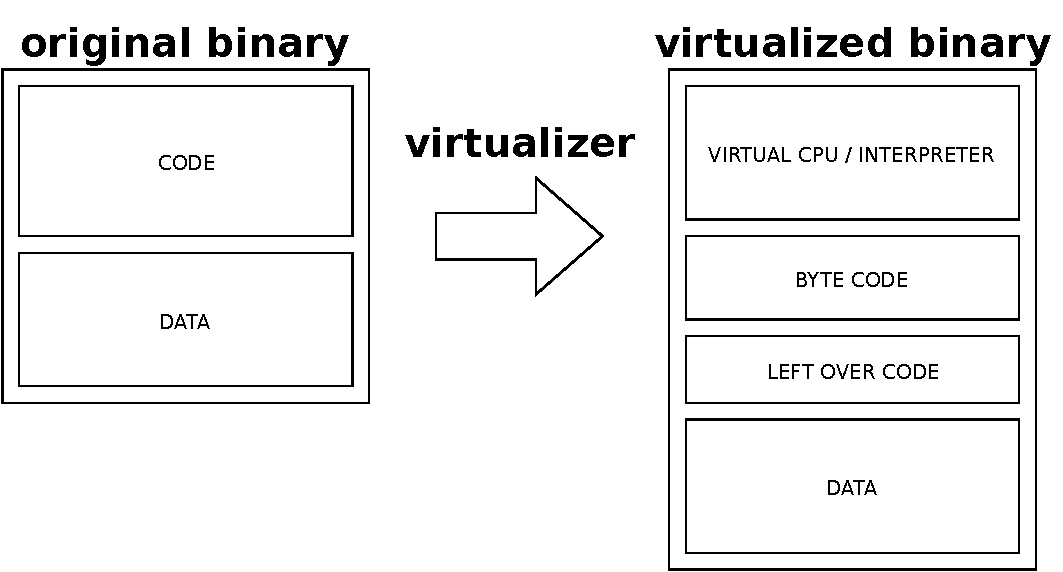
\includegraphics[scale=0.8]{images/ch2/virtualization_process.pdf} 
\caption{The virtualization obfuscation process based on \cite{symantec_clampi}. }
\label{virtualization_process}
\end{figure}

In this section the obfuscation technique, which uses a virtual machine for obfuscation, is described. 
This technique is called virtual machine based obfuscation.
To apply this obfuscation technique the part of the code, which is 
obfuscated, is translated into unique instructions (virtual instructions), which are emulated~\cite{malobfs}
at run time by a virtual machine.
These instructions are then added to the program instead of the original instructions.
Therefore the original instructions are no longer a part of the binary.
This means, that these instructions are not restored during the execution of the
binary.
Instead the functionality of these instructions are represented by the virtual instructions.
In order that the virtual instructions are executed at run time, the emulating virtual machine 
must be added to the binary as well.
To be able to understand the behavior of the obfuscated instructions, both the virtual
machine and the obfuscated code must be analyzed.
These virtual machines are often implemented as switch statements or each instructions 
calls the next instruction according to the current instruction pointer of the virtual 
machine~\cite{rolles}.
The opcodes for the instructions, which are interpreted by such a virtual machine, possibly differ
in every binary.
This means the opcode for the instruction, executing a push instruction, in one binary,
may be used for an addition instruction in another binary. 
This is achieved by a jump table, which assigns the opcode to the instructions, which 
are executed for this opcode.
Therefore this obfuscation technique veils the properties and the behavior 
of the obfuscated code from the reverse engineer.
As well it is not possible to dump the memory to restore the not obfuscated 
instructions~\cite{createvmi}.
With this properties the deobfuscation of virtual machine obfuscation is very time 
consuming and protects the functionality of the obfuscated code against static and
dynamic analysis. 


%%%%%%%%%%%%%%%%%%%%%%%%%%%%%%%%%%%%%%%%%%%%%%%%%%%%%%%%%%%%%%%%%%%%%%%%%%%%%%%
%
% Implementation
% 
%%%%%%%%%%%%%%%%%%%%%%%%%%%%%%%%%%%%%%%%%%%%%%%%%%%%%%%%%%%%%%%%%%%%%%%%%%%%%%%


\chapter{Implementation}
\label{sec3:implementation}

This thesis describes a dynamic approach at virtual obfuscator packed binaries. The approach itself is structured into optimization and analysis techniques and this logical division is reflected in the structure of this chapter.
The first section will give a short overview into the architecture of the framework and the intended ways of use. For a list of all newly implemented features see Appendix A.
Section \ref{sec3:dynana} will explain the techniques used by the dynamic analysis and the theory behind it. This leads to a subdivision of that section into a prerequisites subsection \ref{sec3:prereq}, an optimizations subsection \ref{sec3:opti} and an analysis techniques subsection \ref{sec3:anal}.
Following up will be the automation section, which will explain the grading system of this framework and additional steps towards a more automated work flow.
Concluding this chapter will come the user oriented result presentation and manual enhancement possibilities. This subsection will cover the implemented interaction capabilities of the framework, that allow the user to change the parameters of the analysis and also work interactively with the analysis results.
 
\section{Architectural concept}
The implementation of the application follows a architectural concept which is described in detail in the following part. The actions performed by the applications can be divided into different modules. These modules are separated in the code by packages.

The OCR module holds a java wrapper for the Tesseract - an OCR reader developed by Google. In this module, the process of scanning an invoice pdf is accomplished. Several adjustments, such as language specifications, page turnings and block definitions are made here as well. Section \ref{sec:OCRModule} describes the methods used in here in detail.

...
more descriptions regarding the modules 
\todo{}

Inside the GUI module, all logic for retrieving data and displaying it to the user takes place. The in-depth explanation about the module will be dealt with in section \ref{sec:GUIModule}.

\section{GUI}
\label{GUIModule}
The application provides a graphical user interface to make it easier for users to use the application. Therefore, this module contains classes to define the graphical representation. It follows the paradigm of the MVC concept: \todo{referenz zu mvc}. We extended the MVC framework with a service component. While the controller still manages data from the model to the view (and vice-versa) a service is used that does the actual business logic behind.

Currently, there are three main views to work with:

The Scan Report form enables invoice processing using the OCR module. After the processing part, the data is shown so that the user can edit information, add missing information or information that have been falsely identified by the OCR reader.
When everything is correct, the data is stored in the database pressing "save". During this process, the ZugFerd-Module extends the invoice scan, adding the ferd-information to it after validation.

The Finder form enables searching the database providing key-values such as names, dates or values. If completely left blank, all data is shown.
Additionally, a button enables saving the invoice to the pc. This way older invoices can be retrieved again.

The Report form enables additional comfort functions such as excel-reports regarding the data stored in the database, balances for specific companies and others.

In addition to that, the application provides several setting options where the user can change database access information, the preferred language in the application as well as the language used during the ocr process, the export and import of the database (backup) and more.

\begin{figure}[htp]
\centering
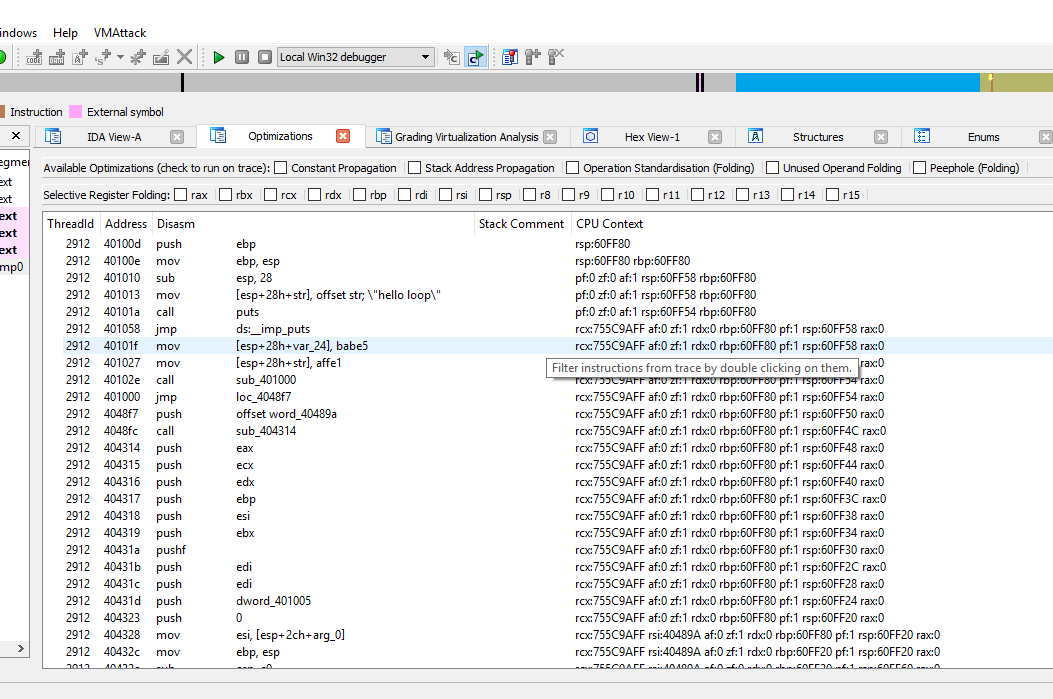
\includegraphics[scale=0.40]{images/ch3/optimizations1.png}
\caption{Trace Presentation and Interactive Optimization Viewer.}
\label{opti1}
\end{figure}

\subsubsection{Constant Propagation} 
Constants are propagated where possible. Basically this means registers are switched with their values and offsets which can be computed will be computed.\\
Initially this optimization differentiates behavior for single operand instructions and two operand instructions. Instructions without operands are ignored by this optimization.
Most single operand instructions are disregarded. 
First implementations naively switched every register with its CPU context value but it became clear very early that this is a rather cumbersome approach. 
For example if in the instruction \code{push eax} the register is replaced with its current value \code{1234} it is debatable whether it promotes a better understanding for the reverse engineer or not. 
For this reason it was decided to mostly ignore single operand instructions, as most replacements were not judge to improve readability of the trace. There are two exceptions however:
\begin{itemize}
\item{Instructions using a computation with a register or a memory address.}
\item{Instructions using a register for addressing.}
\end{itemize}
A lot more work is done on two operand instructions. In the optimization context handled cases are register access, memory location access and computation.
The basic differentiation is between reading and writing instructions, as reading instructions have to be processed more often than writing instructions.\\
If an instruction reads a register, the register name is replaced with the read value taken from the CPU context. This improves readability, as the reverse engineer does not have to look up the value for the register anymore.
If on the other hand an instruction writes a register, the register name is not replaced. This would have a negative effect, as the reverse engineer would need to check the CPU context if he would want to know which register was written.\\
A special case consists of computations with a register. For example dereferencing the address \code{[eax*8+offset]}. 
As all necessary information for computation of this address exists, it is computed and the final result will be \code{[value]}, where value is the computed equivalent of \code{eax*8+offset}. The register value is taken from the CPU context as before.\\
This is somewhat of a trade-off, as the reverse engineer can see which memory address is used, however the information about how this address is computed is lost.
Before the optimization it is clearly visible, that offset is a relative point for addressing something. In the context of VM obfuscation it might be for example a point inside the `jump table'\footnote{A jump table is a construct to transfer program control to another part of a program using a table of branch or jump instructions.} 
In the most simple case this will be the base address of the jump table. Note, that jump tables are also sometimes referred to as branch tables. 
The value in eax is then used to decide an offset inside this jump table. Such information is then lost if the value is computed by the constant propagation optimization.
We do not consider this to be a grave loss of information however. This is due to the static analysis of IDA being available in a neighboring window. If a reverse engineer desires to get informations about the addressing scheme of the VM he still can do so for example in the IDA Graph, which is the determined control flow graph for the current binary. \\
The same procedure is followed for memory locations. If memory locations are a result of computations, they usually will be computed, as all information should be available.
Pointer indicators are preserved if possible, as is other relevant information. 
If possible the optimization only replaces the part which can be computed and leaves the rest of the instruction as it is.


\subsubsection{Stack Address Propagation}
This optimization enables stack comments in the trace. Every time a stack address is read the value on that stack address will be available as stack comment to the reverse engineer.
As stack information is not part of the instruction trace memory locations can not simply be read from the trace. But an instruction trace itself has all the stack interaction which is required to recreate the some stack fragments.\\
At the beginning of this optimization a shadow stack is created. 
Then the trace is read and every interaction with stack is logged. If for example \code{1234} is written on the stack the same operation is done for the shadow stack. This way the stack at execution time can be recreated.
If a memory location is then read, the shadow stack at this particular time in execution is used to create the stack comment, which tells what value is currently provided in said location - \code{[memory address]=value}.
This improves the readability as the reverse engineer can see right away which value is currently in the relevant memory location.



\begin{figure}[htp]
\centering
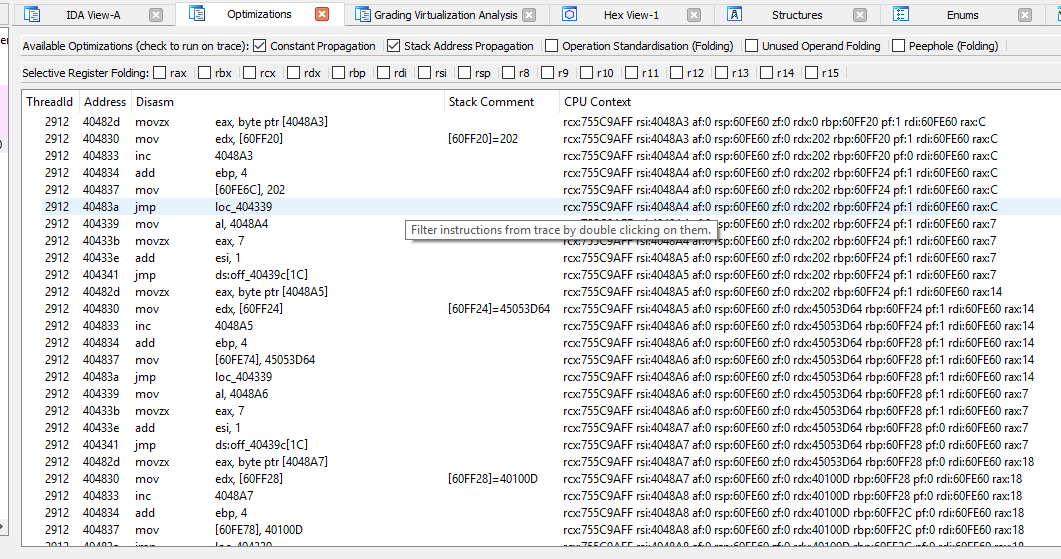
\includegraphics[scale=0.40]{images/ch3/optimizations2.png}
\caption{Instruction trace after the two propagation optimizations.}
\label{bothprop}
\end{figure}

\paragraph*{Propagation vs. Folding}At present, two propagation optimizations are supported by the framework. The focus of propagation optimizations is to make information that is known at the time of the analysis easier available to the reverse engineer. 
In the case of constant propagation for example we already know the register values from the CPU context or can compute memory locations and thus can replace replace some registers or simple computations with their corresponding values. 
The reverse engineer does not need to lookup or compute every value now, since most will already be clear from the instructions themselves. 
As such propagations can be considered as safe optimizations which have the focus on enriching the trace with available but maybe difficult to get information.
A trace after the application of both optimizations can be seen in figure \ref{bothprop}. \\
Folding optimizations however have a different focus. They already perform trace reducing operations, resulting in a smaller trace to analyze. 
They can be quite powerful, reducing the trace by a very high percentage but also carry a risk of leaving out crucial information. As such they should be applied with care.
Additionally some folding optimizations might require the the propagation optimizations to have already been applied to the trace.

\subsubsection{Operation Standardization}
This optimization is used to create a common ground for the optimizations. The goal is to transform instructions without changing the outcome of the operation. 
An example for this is the equivalence of \code{add esp, 1} and \code{inc esp}. Both operations result in the same outcome and can be referred to as semantically equivalent. 
Yadegari et al. call these transformations semantics-preserving transformations in \cite{DBLP:conf/sp/YadegariJWD15} and use symbolic execution to find such transformations. 
VMAttacks approach uses dynamic analysis and pattern matching to find certain patterns and simplify them.

\subsubsection{Unused Operand Folding}
This optimization purges operands and computation results from the trace if they are not used. 
The optimization algorithm starts at every write instruction and traverses the trace. 
If a read instruction is found that uses the previously written value the algorithm stops and the next write instruction is viewed. 
If no read instruction until the end of the trace is found or if a write instruction is found that overwrites the previous value before it is read the initial trace line is deemed irrelevant and thus removed. \\
To mitigate removal is is enough to find a read instruction or computation on even the smallest part of a register. If a value was written to the \code{rax} register and only the \code{al} or \code{ah} registers\footnote{The \code{ah} and \code{al} are the higher and lower bytes of the \code{ax} register, which is part of the \code{eax} register, which in turn is part of the \code{rax} register.} are read this will stop the algorithm and the search will continue with the next write instruction.


\subsubsection{Peephole Optimizations}
The peephole optimization consists of pattern matching algorithms. 
The trace is traversed for specific patterns which are then replaced, transformed or deleted if deemed unnecessary. 
Currently supported patterns consist of a frequency based pattern matching, specific manually defined multi-line patterns flagged as irrelevant and propagation dependent removal.\\
Frequency based pattern matching removes the repeating trace lines with the highest frequency. The logic behind this removal lies in the architecture of the VM interpreter. 
The abstract structure of the VM interpreter is that of a switch statement. 
Hence there is a part responsible for fetching and evaluating the next byte from the byte code that will be traversed in each execution cycle. 
Then there are the separate switch cases, that will be traversed much less frequently, since their traversal depends on the currently evaluated byte.
Since the main purpose of these optimizations is not to decipher the byte code's relation with the interpreter but instead to filter the relevant instructions, the fetching and evaluation of the byte code can be left out to reduce the trace considerably. \\
The propagation dependent peephole will remove trace lines that provided the necessary information to perform the propagation optimizations but are not needed anymore.
This includes for example the stack to register interaction, i.e. read instructions for memory locations. This does not include write instructions to the stack, as these instructions are the result of a computation and for some instructions might leave out critical information, e.g. the `lea' instruction. 

\subsubsection{Additional Filtering Capabilities}
Aside from the three folding optimizations VMAttack offers additional filtering capabilities.
First of all, the reverse engineer can filter complete registers from the trace. Filtering the eax register from the trace accomplishes the complete removal of all lines containing the eax register in the instructions field.\\
This accomplishes two intended behaviors. First, if the constant propagation optimization was not run, the trace will be reduced quite heavily. All instructions using the eax register will be removed. 
This can be quite useful to filter registers that have nothing to do with the value computation inside the VM itself. Should a reverse engineer determine, that i.e. the ecx register is only used for obfuscation purposes it can thus easily be removed.
Another use case would be the VM program counter. If a reverse engineer does not want to map the byte code to executed instructions but instead wants to quickly filter unique instructions, this provides a quick interface for that solution. 
The VM program counter register can thus be easily removed, reducing the trace considerably and thus the analysis time needed for deobfuscation. \\
The second intended behavior takes place if the constant propagation optimization has already been applied to the trace. 
The filtering of a register will then again remove all trace lines performing an operation on said register. But all trace lines using a value from that register will not have the register name in them anymore, due to the constant propagation! 
Thereby this constitutes a safer way of removing registers from the trace. 
Safer means in this context, that if a value from the register was used, the register name in this trace line will have been replaced by that value, hence the line will not be removed and thus the information, how values came to be will be preserved.\\
Same applies to the filtering approach of instruction filtering offered by this Trace Viewer. This filtering approaches behavior is influenced by the optimizations constant propagation and operation standardization.
As the approach filters all instructions that equal the double clicked instruction, the effectiveness depends of the number of available and recognized equal instructions. 
Operation standardization improves this number, due to the instruction transformations creating a common ground for equivalent operations.
Constant propagation on the other hand reduces this number, due to some register names being replaced with their current CPU context. This turns once equal instructions into differing ones, if the CPU context for that register was different.

\paragraph*{Limitations of the Optimization Approach} The optimization approach is rather powerful, as it adds additional information to the trace and allows for filtering nearly anything unwanted. 
However this requires the reverse engineer to know what kind of information is unwanted before the filtering can be executed in a useful way.
The filtering done by the folding optimizations greatly relies on recognized patterns and useful considered optimizations. This usefulness relies heavily on the analysis done by the framework maintainers and as such is not a sustainable solution once obfuscation authors decide to target this analysis technique. 
From this arises a danger, that obfuscation can be designed quite easily to counteract folding analysis optimizations or even make them leave out critically important trace lines.
  

\begin{figure}[htp]
\centering
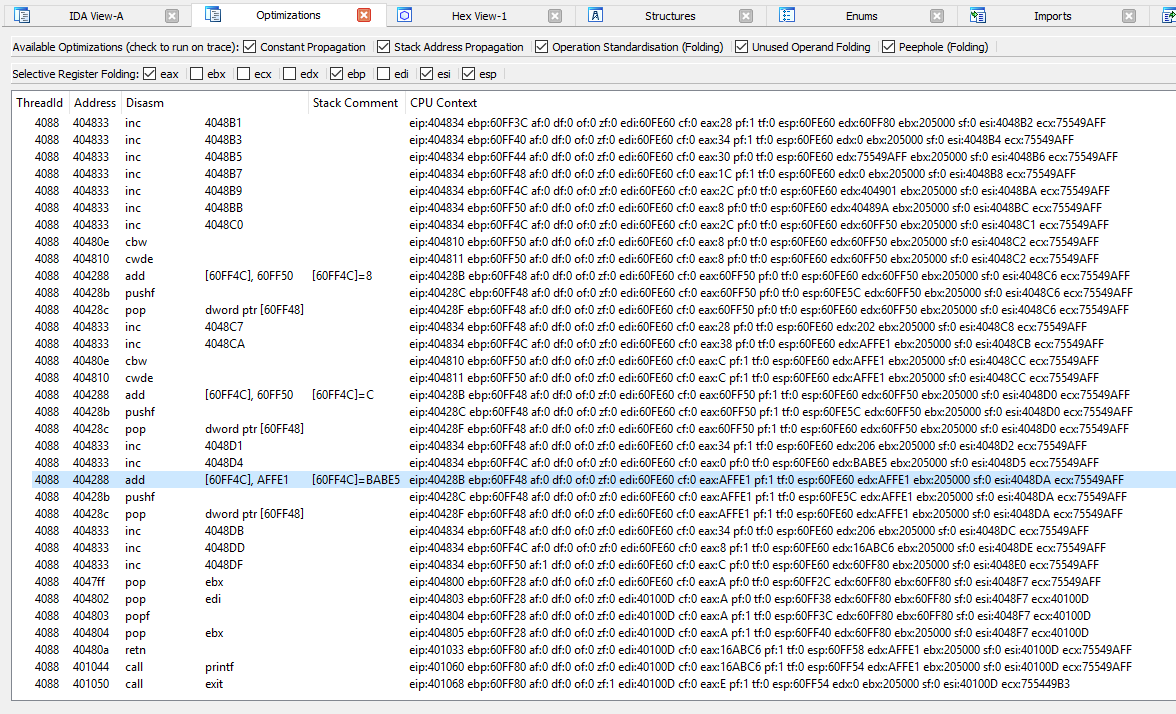
\includegraphics[scale=0.48]{images/ch3/optimizations_success.png}
\caption{Instruction trace after all five optimizations have been applied.}
\label{opti3}
\end{figure}

\paragraph*{Optimization Result}The result of a complete application of the five optimizations and some additional register folding can be seen in figure \ref{opti3}. On an abstract level the trace folding optimizations, especially the peephole optimization, coupled with the additional filtering capabilities can be already considered as dynamic anti-virtualization technique. 
Both, the input/output analysis and the clustering analysis traverse the trace and remove unwanted instructions. 
The same can be said for the folding optimizations. The only difference being the bigger manual interaction needed for the additional filtering capabilities. This increased manual interaction however also offers a seasoned reverse engineer to extract the trace lines deemed important more easily. 

\subsection{Dynamic Analysis techniques}
\label{sec3:anal}
\subsubsection{Input/Output Analysis}

The input/output analysis is a combination of dynamic execution of the binary coupled with simple value level taint tracking approach. It is an VM architecture independent approach and will work even on the most obscure VM architectures. The goal of this analysis is to find a connection between the VM input parameters and its output parameters.\\
The prerequisite of using this technique is a generated instruction trace, which is the starting point of this algorithm. The generation of such a trace has been covered in the prerequisite section of this chapter and will not be discussed again.\\
If not already enforced the two propagation optimizations detailed in the last chapter will be applied to the trace before further optimization takes place.
This is not necessary for the optimization itself, however it is crucial for the result presentation.
As the optimization is filtering the relevant trace lines from the trace, viewing the result can be quite confusing without the stack values propagated because the reverse engineer does not know which values are written in a read memory location. \\
After the two optimizations the actual analysis step can proceed. First, the VM function input values are either extracted from the trace or if the trace was generated they are read from the framework environment.
Next the function output parameters are determined. To this extend all registers popped from the stack before function exit are considered VM output parameters.\\
The next analysis step is to try and ascertain whether there is a relation between these values. To accomplish this, for each result register the analysis backtraces how the result value came to be. First, the result value is backtraced on the trace to its corresponding stack address. Next, the analysis determines how the value saved on this address came to be. The algorithm backtraces the value to its point of oringin which will be either a memory address or a computation.\\
If the values point of origin is a computation the algorithm is repeated for the two values used in the computation. This ensures, that composed values are extracted correctly, meaning all trace lines regarding the computation are also traced back to the point of origin for the values used in the computation. 
A visual representation of this approach can be seen in figure \ref{io_algo}.

\begin{figure}[htb]
\centering
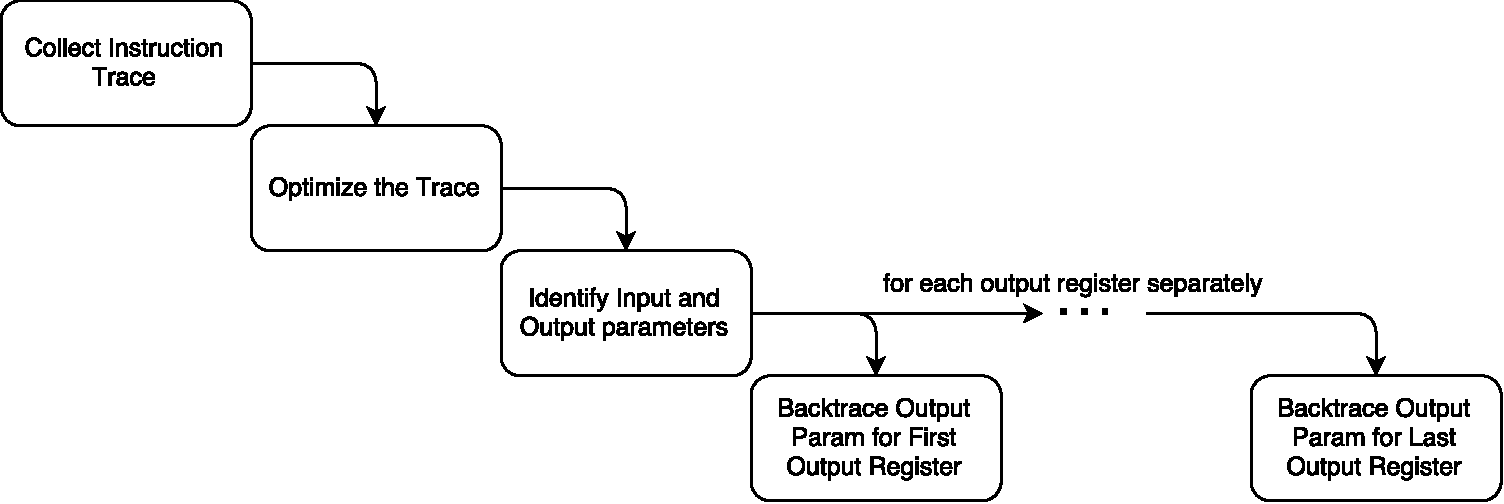
\includegraphics[scale=0.60]{images/ch3/InputOutput_algo.pdf}
\caption{Input Output based backtracing algorithm.}
\label{io_algo}
\end{figure}

The result of this analysis can be seen in figure \ref{io_result}. The reverse engineer is presented with the VM's output registers. 
For each register the backtrace of the result value is provided. The reverse engineer can get the necessary information of how a value came to be and whether this value depends on the input parameters for the VM function or not.
Coloring is used to diffenretiate between the input and output values, for the coloring scheme see section \ref{sec3:UI}. 

\begin{figure}[H]
\centering
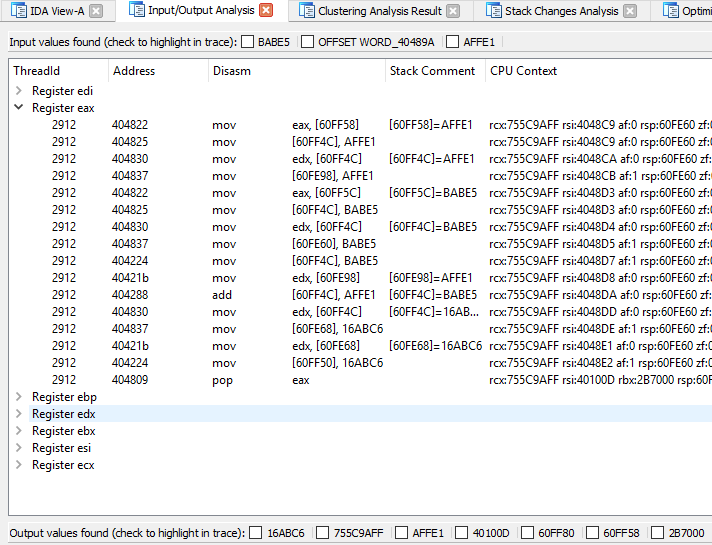
\includegraphics[scale=0.62]{images/ch3/InputOutput1.png}
\caption{Result of the Input/Output analysis.}
\label{io_result}
\end{figure}

\paragraph*{Limitations of Input/Output Analysis.} This analytic approach backtraces the output values to their atomic components. 
If these components are not dependent on the input parameters to the function this analysis will not yield significant results.
The atomic values can be found but if they stand in no relation to the input values the significance of found values does not necessary reveal much about the inner workings of the obfuscated function.
As such the use case is primarily intended towards obfuscated functions which perform some kind of transformation on the input values, i.e. license key checkers or secret computations for example trademarked algorithms.\\
Nevertheless to counteract this analysis and even hide functionality, obfuscation on an abstract level can simply use this output orientation to compute a meaningless result from input and return it while additionally running a hidden routine which is not input dependent.
Such an approach would not be detected by this analysis technique as only input and output parameters are considered taint values and the rest of the functionality is considered irrelevant.

\subsubsection{Clustering Analysis}
The clustering analysis is a combination of dynamic analysis, pattern matching and a heuristics based approach. It is a deobfuscation technique using the looping execution flow of the virtual machine against itself by detecting groups of constantly repeating instructions. This analysis technique is useful for every VM architecture that has repeating instructions as part of the execution routine. \\
As dynamic analysis clustering is performed on a previously acquired instruction trace. The algorithms first step is to obtain an instruction trace.
The acquisition remains the same for all dynamic analysis techniques and as such was already covered in the previous section \ref{sec3:prereq}.
There are two possible scenarios for optimizations in the clustering analysis. The default case is the use of the two propagation implementations which are enriching the trace with additional information. In the customized case the reverse engineer decides himself which optimizations are applied to the trace (propagation and folding are possible) and starts the clustering algorithm afterwards.\\
The address based clustering approach consists of several clustering rounds which are applied to the instruction trace.
In each clustering round the trace is traversed and for every address and its neighbor the trace is checked to have the exact same constellation of addresses. If this same constellation exists and the occurrence of this constellation is higher or equal to the `cluster heuristic' a cluster is created. The `cluster heuristic' is a user definable border to determine how many occurrences it takes to be considered a cluster. The default `cluster heuristic' is 2.
This prompts four possible cases:
\begin{itemize}
\item{The first address and the neighboring address are both single trace lines.}
If this is the case a new cluster is created consisting of the two trace lines. 
\item{The first address is a single trace line and the neighboring address already belongs to a cluster.} In this case the single address trace line is added to the cluster.
\item{The first address belongs to a cluster and the neighboring address is a single trace lines.}
\item{The first address and the neighboring address both belong to clusters.} This case prompts a cluster merge resulting in a bigger cluster being created, consisting the single lines from both clusters.
\end{itemize} 
Consecutive rounds will obviously result in bigger and bigger clusters. There is a threshold however, after which all repeating instructions have been identified and added to clusters.
Repeating clustering rounds until this threshold is reached is commonly referred to as greedy clustering and is also the default case of this analysis. If a clustering round yields no length increase for any cluster the algorithm stops.
If however greedy clustering is disabled, then the user specified amount of rounds is executed.


\begin{figure}[htb]
\centering
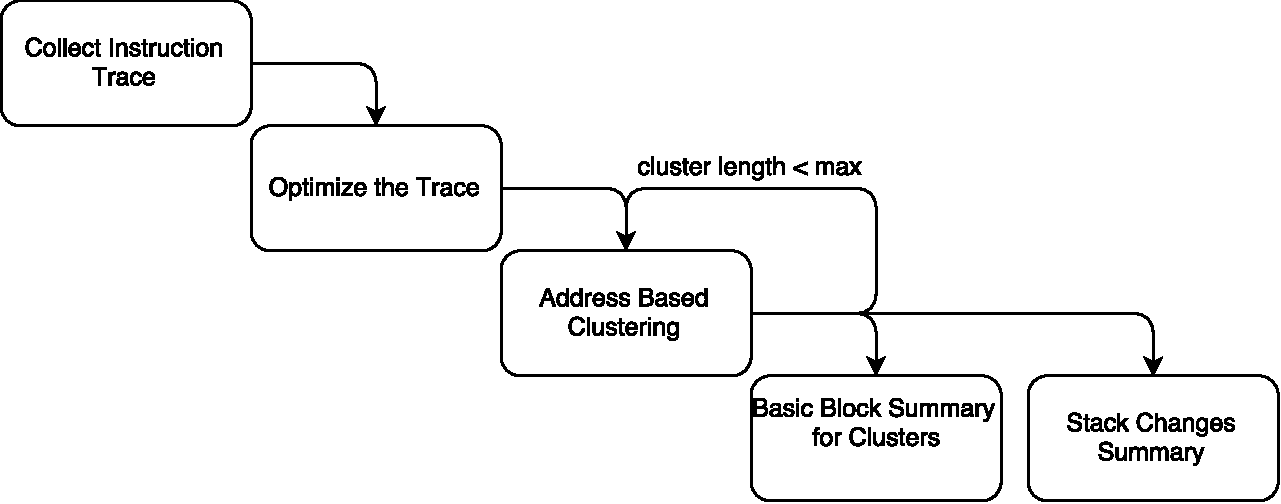
\includegraphics[scale=0.75]{images/ch3/clustering_algo.pdf}
\caption{Address based greedy clustering algorithm.}
\label{clu_algo}
\end{figure}

There are currently two ways a clustering analysis result can be presented to the reverse engineer, with or without basic block display.
If basic block display was not deactivated in the settings interface the basic block division and the basic block summary are computed and displayed.
This enables the reverse engineer to remove basic blocks, clusters or trace lines. 
Additionally, the summary for a basic block allows for a quick overview about relevant operations, relevant memory allocations and addresses contained in this basic block.
If basic block display was deactivated, only the clusters and trace lines are displayed within the clusters. This view disregards basic block boundaries and enables the reverse engineer to see a representation with focus on repeating clusters instead of repeating clusters and basic block by removing the middle abstraction layer. 
\newline
Additionally the stack tracing is also presented in a separate viewer. The reverse engineer can thus determine quite easily what values were saved and which operations were computed with which stack addresses. 
The stack trace is computed during the clustering analysis' basic block summaries and requires the constant propagation and stack address propagation optimizations to be applied to the trace. \\
All used stack addresses are regarded and presented with all values that were saved on this stack address during execution. If the value was not moved or pushed onto the stack, or in a computation prior to be moved on the stack the computations instruction and second value are displayed as well.\\
Finally, after result presentation the reverse engineer can decide to remove several most occurring clusters, or decide for each cluster type whether to keep it or to remove it. The interactive nature of the result presentation allows for a highly tailored solution as to which clusters and or basic blocks to keep and what to remove.

\begin{figure}[H]
\centering
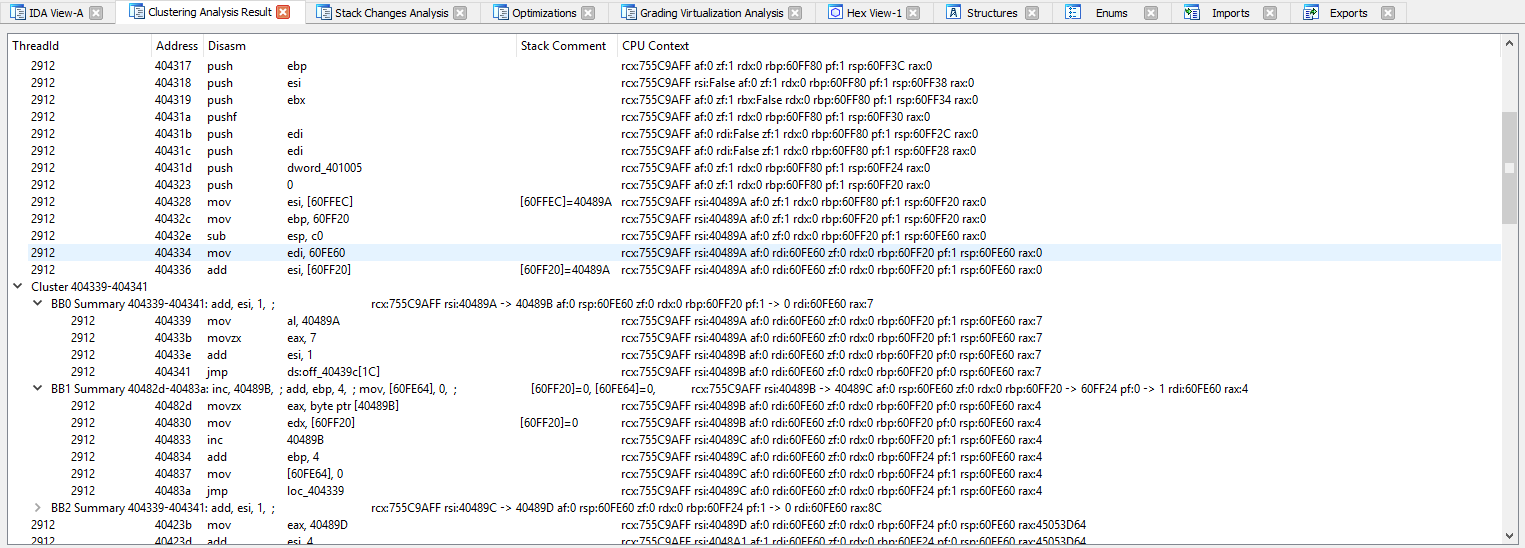
\includegraphics[scale=0.50]{images/ch3/clustering1.png}
\caption{Result of Clustering Analysis with basic block display enabled.}
\label{clu_result}
\end{figure}

\paragraph*{Limitations of Clustering Analysis} The clustering analysis itself is not an analysis technique that removes lines from the trace per se. Rather the reverse engineer is presented with a different view on the instruction trace.
What the analysis does however is to enable the reverse engineer to quickly remove clusters.
With only a few mouse clicks the top frequent clusters or even all of them can be removed, which requires the reverse engineer to know exactly which clusters need to be removed and which are should be left.
This results in a higher manual interaction needed to make the analysis result meaningful. 
This trade-off while being a limitation is necessary however, as the other alternative would be the default removal of clusters, but this would assume, that clusters do not hold any relevant functionality.
As this was not true for any of the test cases discussed in the evaluation the current approach was considered best, as it would harm analysis tremendously if information was left out irreversibly.

\section{Automation}
\label{sec3:automation}

Automation is an important focus of the plug-in. There were several smaller work flow improvements in regards to automation and the fully automatable grading analysis system.\\
Two newly introduced key automation techniques are the dynamic and the static VM context search. These are highly important, as without them the static analysis is only possible by manual invocation, which would mean additional analysis work for the reverse engineer.
Both techniques extract these values from the context they are given. For the static VM context search this is done without executing the binary, for the dynamic VM context search a instruction trace is used.\\
\subsection{Virtual Machine Context}
\paragraph*{Definition: VM context}\emph{The virtual machine context, short VM context, is an object consisting of four integer values:
\begin{itemize}
\item{byte code start address}
\item{jump table base address}
\item{byte code end address}
\item{virtual machine function start address}
\end{itemize} }

%%% Automated static VM context search
\subsubsection{Static VM Context search}
The static search first determines the virtualized segment of the binary. 
As the virtualized segment can have more than one function, usually at least two functions will be present, the VM interpreter itself and additionally a small calling stub, which pushes necessary information onto the stack, such as a pointer to the byte code and possibly some initial values for the VM function. 
To differentiate these two functions their size is used as the main criteria, based on the assumption that the VM function will be bigger in size. 
After the VM function is determined the base address of the jump table needs to be found.
The last two remaining values are the byte code start and end. Due to the automation functionality of the static deobfuscation function the byte code end does not really need to be determined. Instead the end address of the virtualized segment is enough already. 
The byte code start is determined via the VM calling stub. As mentioned earlier, the stub is responsible for setting up the VM environment and creating a stack the VM can work with. This is where the pointer to the byte code for the VM to interpret is pushed onto the stack. VMAttack uses this to identify the byte code.

\paragraph*{Limitations of Static Search} The static search is based on assumptions about the structure of the virtualized segment and the VM function. If these assumptions are not met for example due to obfuscation of these parts, the analysis will fail.\\
One such assumption is that the VM function is the biggest function in the segment. As an obfuscation measure a malware author could try to split the VM function into two or use two different VM interpreters and two byte code locations.
This would result in an unsuccessful search for the VM function, additionally it would hamper the byte code search, as without the knowledge that there are two different VM functions the analysis algorithm does not know to look for two different byte code starting points.
Currently such a problem could only be mitigated with the manual interaction of the reverse engineer with the framework. 
The work around could be that the reverse engineer would manually relegate the VM context values via the settings interface and invoke the static deobfuscate function twice, once for every VM function with its corresponding byte code.

%%% Automated dynamic vm context search
\subsubsection{Dynamic VM Context search} The dynamic counterpart uses the same abstract approach as the static but with a completely different implementation. 
First and foremost the dynamic approach uses the instruction trace and not the static binary, which provides a lot more information. 
The VM function address is determined directly via the executed mapping of push to pull instructions. The function with the most mappings will be considered the VM function.
Contrary to the static search this decision is verified however. The VM Segment is also searched for the biggest function and then a verification of the VM function takes place. 
If the verification fails, the reverse engineer is asked to choose the most fitting alternative.
The base address of the is determined from the instruction trace as well. 
First the repeating jump offsets are counted which happened inside the VM function. The most common offset is then examined statically to be the base of the jump table and if this is not the case it is corrected to the base.
The byte code start is determined dynamically by examining the function parameters provided to the VM function.
This is then checked with IDAs Code and Data detection engine, whether the provided pointer really leads to a data address. 
The code end is again assumed to be the virtualized segments end.

\paragraph*{Limitations of Dynamic Search} As seen previously with the static approach the dynamic search relies on assumptions concerning the architecture of the VM. 
If this architecture is changed too much these assumptions might not be true anymore and as such the analysis algorithm will fail.
For example the approach at the base address assumes, that the most common jump offset does indeed use the jump table. 
This is a fair assumption given the structure of the VM interpreter, which is quite similar to a switch statement. 
However this can be fatal if enough obfuscation is used and the structure of the VM interpreter does not resemble that of a switch statement anymore. 

%Automated Analysis

\subsection{Grading System}

The grading system analysis is a combination of all available analysis capabilities(static and dynamic) of VMAttack with additional pattern matching mechanisms. The basic principle is, that each trace line is initialized with a certain seed value, depending on the uniqueness of the trace line. 
This value is in turn upgraded or downgraded after each analysis run, depending on the importance an analysis assigns to this trace line. 
Additionally, after each analysis run a pattern matching upgrade or downgrade occurs for certain predefined patterns.

\subsubsection{Initialization}
As dynamic analysis capabilities are used the first algorithm step is obtaining an instruction trace. This procedure does not differ from the other dynamic analysis techniques and thus will not be explained again. \\
After the acquisition of the instruction trace the trace lines are initiated with their starting grade.
A lines starting grade is determined by the lines uniqueness, where the more unique a line is, the higher the grade will be. To accomplish this outcome the occurrence of all line addresses is counted. This produces an occurrence to address mapping and allows for a classification of occurrence levels.
These levels constitute the initial grades in reversed order. To clarify consider the following example:

Lets assume we have an instruction trace with 30 trace lines. If we have 9 unique addresses, three addresses encountered twice the three addresses encountered five times, the result will look as follows:
\begin{itemize}
\item{9 trace lines with addresses encountered once: \textbf{grade 3}}
\item{6 trace lines with addresses encountered twice: \textbf{grade 2}}
\item{15 trace lines with addresses encountered five times: \textbf{grade 1}}
\end{itemize}

This coupling to the occurrence levels of a trace makes the initialization process highly dynamic. As can be seen in the example the initialization process does not take into account how many times an address was encountered, only that a difference exists.
This is a direct result of the working dynamic of the VM. The VM constantly fetches, decodes and executes byte code from memory. This results in some instructions being repeated a numerous number of times, while others executed only once. 
However, depending on the VM some data transformations and computations are carried out by the \textbf{same} instructions from the fetch-decode-execute cycle. This means, uniqueness of an instruction is \textbf{not} the only factor determining the importance of a trace line. 
Hence the difference in occurrences is taken into account as the grade itself but not the number of occurrences.

\subsubsection{Input/Output Analysis Grading Step}
The next grading step is modeled after the input/output analysis of VMAttack. The algorithm assumes the default case, that all output registers are considered important and obtains the input/output relevant trace lines for every output register.
These trace lines are then upgraded with the defined value importance for the input/output analysis in the grading system.

\subsubsection{Register Usage Grading Step}
As previously mentioned a VM constantly fetches, decodes and executes byte code from memory. This is usually done by acquiring the VM program counter from the stack by pushing or moving it into a register, evaluating it and using it to compute the offset for the next byte in the byte code. 
Since the dynamic approach of VMAttack is to filter fetching and offset computing instructions, this analysis step determines from the trace which registers are used for for these two steps and lowers the grades for all trace lines containing these registers.

\subsubsection{Clustering Analysis Grading Step}
This step relies on the clustering analysis results to increase grades for unique lines and decreases the grades of repeating lines. 
However not all repeating instructions are decreased, but merely the most frequent occurring ones, to reduce the grades of fetching instructions even further.


\subsubsection{Optimization Grading Step}
The optimization grading step uses the available optimizations to determine important instructions. The application of all available optimizations results in a highly reduced trace. 
For every line in the reduced trace the grade for the corresponding line in the original trace is raised by the specified importance value.

\subsubsection{Static Deobfuscation Grading Step}
At the end of the analysis the result from the static deobfuscation is integrated into the grade. 
Because the abstract commands from the static deobfuscations' result are presented in the IR language, the are first mapped into assembly instruction for the x86 architecture \footnote{VMAttacks static deobfuscation only supports a subset of most frequently used x86 instructions at the moment. As such only this subset of x86 instructions can be recovered from the IR language and used to improve trace line grades.}. 
Afterwards these instructions are looked for in the trace and if a match is found the grade is raised by the specified importance value for static analysis.
If the instruction could not be found in the trace it is disregarded.

\subsubsection{Summary Grading System}
This design results in high robustness of the automated analysis, as the overall grade of a trace line consists of several grading steps and one failing analysis will not impact the grade greatly.
All the used analyses algorithms are automatable which ensures very low levels of user interaction. The only crucial user input are the importance weights if the default values are not preferred.
As dynamic analysis techniques are faster than concolic techniques the speed of the analysis is considered high, although this strongly depends on VM architecture, trace length and other factors like additional obfuscation methods. 
However, some analysis techniques can still be enhanced in terms of speed by applying a better approach at multi threading. 
As VMAttack is a prototypical implementation enhanced multi threading techniques were disregarded to ensure best possible stability in the provided time frame for the implementation. As a result the current multi threading concept is quite simple and favors stability over speed.
Additionally a better result can be achieved by countering the known weaknesses of certain analysis steps with pattern matching. Known patterns are already applied after each analysis step, for example to reduce the grades of unique lines not belonging to the VM. 
With additional testing, more weaknesses can be determined which will in turn help improve the result even further.\\
After a successful grading analysis attempt the user is presented with the result in the grading analysis viewer. The result consists of necessary trace information and the grade for each trace line. The reverse engineer can simply choose which grades will be displayed in the viewer and thus filter the relevant instructions as needed.

\begin{figure}[htp]
\centering
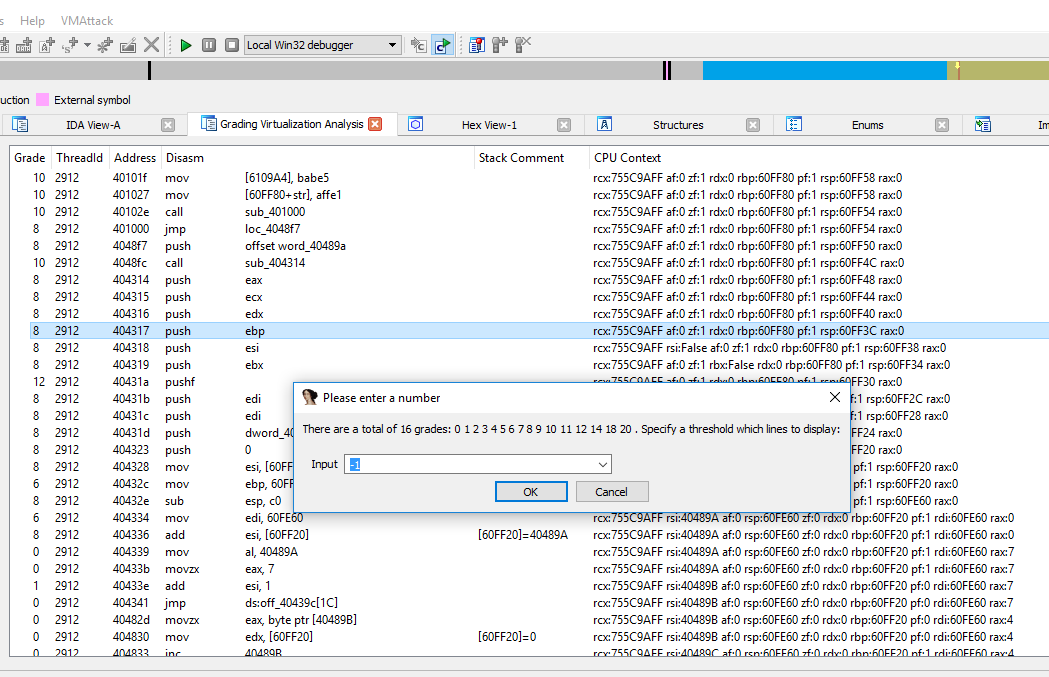
\includegraphics[scale=0.40]{images/ch3/grading3.png}
\caption{Result of the Grading Analysis.}
\label{result_grading}
\end{figure}


\section{Interactive Result Interaction}
\label{sec3:UI}
\subsubsection{Optimizations Analysis View}
\todo{}
\begin{figure}[H]
\centering
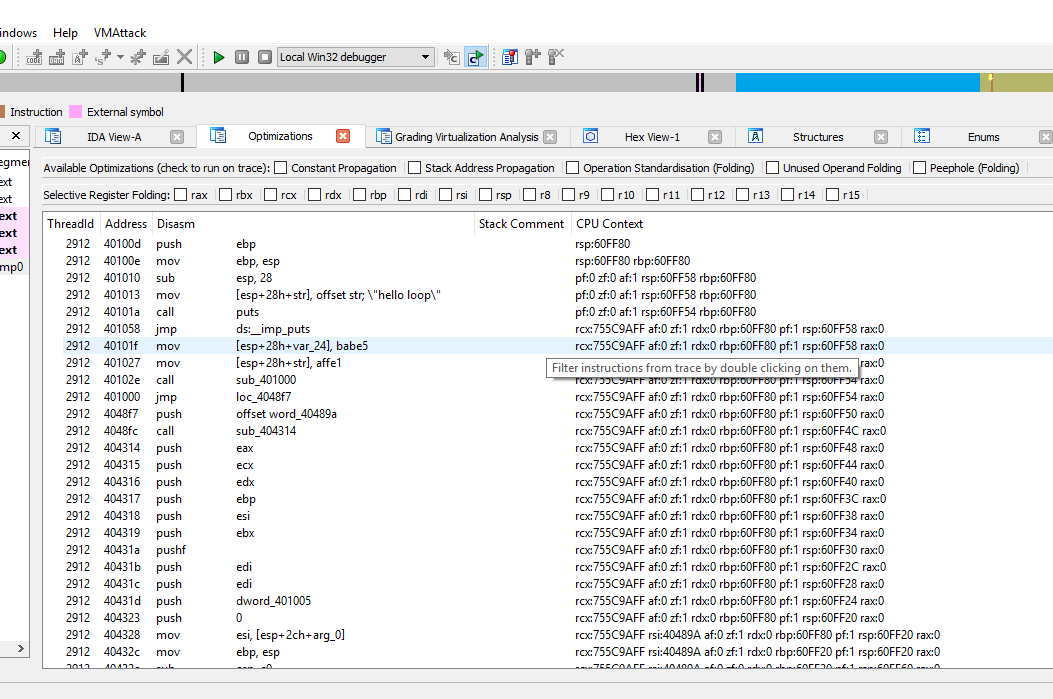
\includegraphics[scale=0.40]{images/ch3/optimizations1.png}
\caption{Abstract VM CFG created from the deobfuscated byte codes.}
\label{}
\end{figure}

\subsubsection{Input/Output Analysis View}
\todo{}
\begin{figure}[H]
\centering
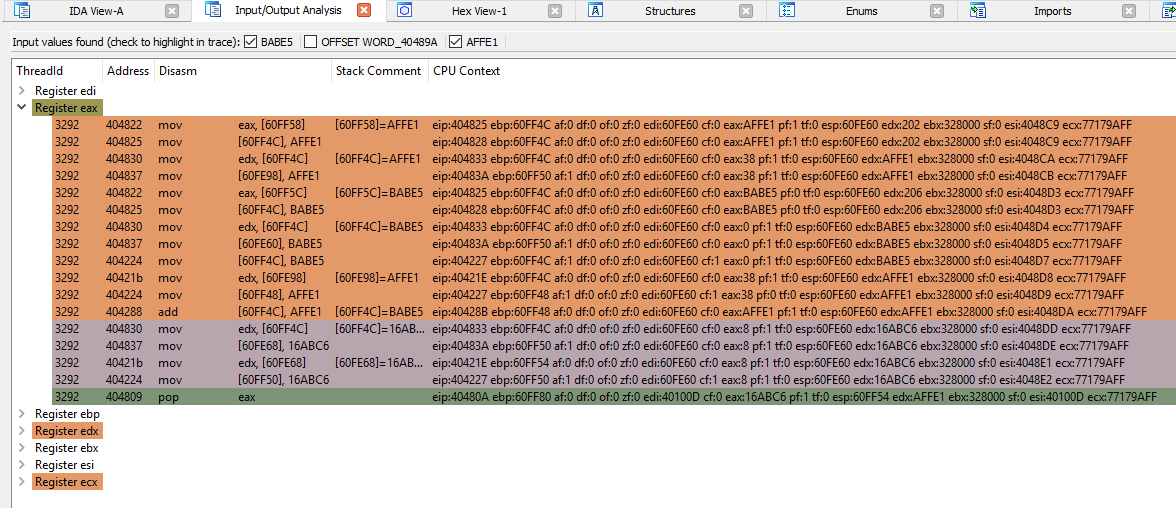
\includegraphics[scale=0.60]{images/ch3/InputOutput3.png}
\caption{Abstract VM CFG created from the deobfuscated byte codes.}
\label{}
\end{figure}

\subsubsection{Clustering Analysis View}
\todo{}
\begin{figure}[H]
\centering
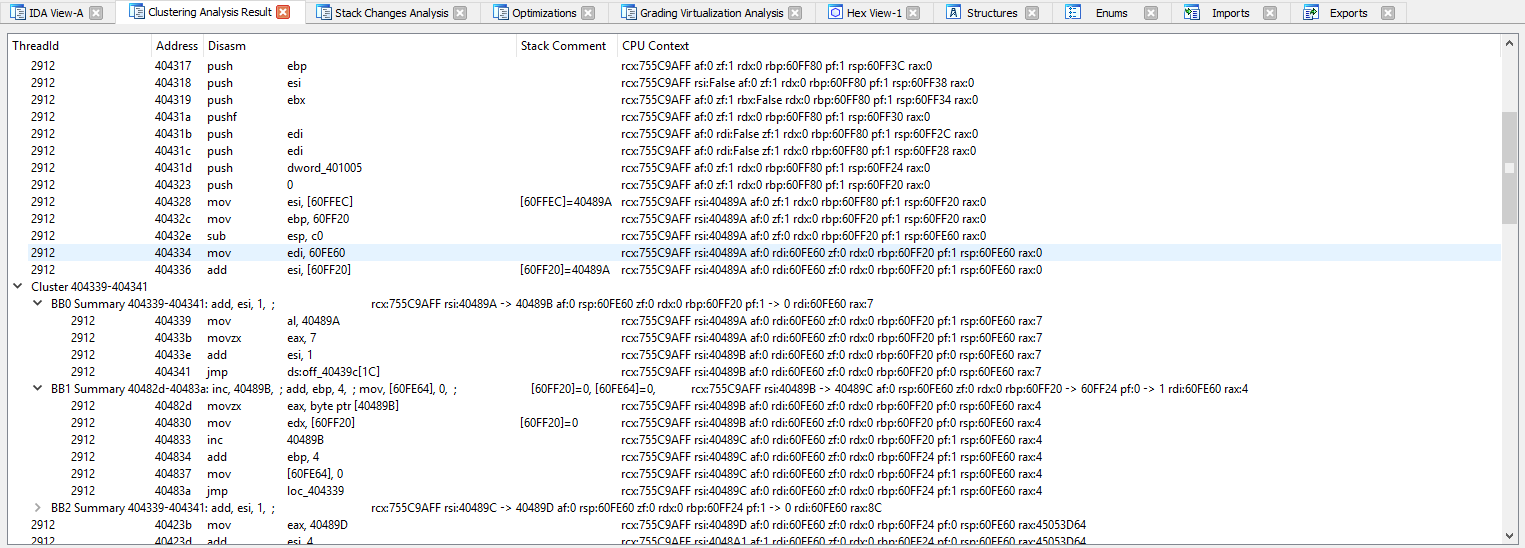
\includegraphics[scale=0.50]{images/ch3/clustering1.png}
\caption{Abstract VM CFG created from the deobfuscated byte codes.}
\label{}
\end{figure}

\subsubsection{Stack Changes View}
\todo{}
\begin{figure}[H]
\centering
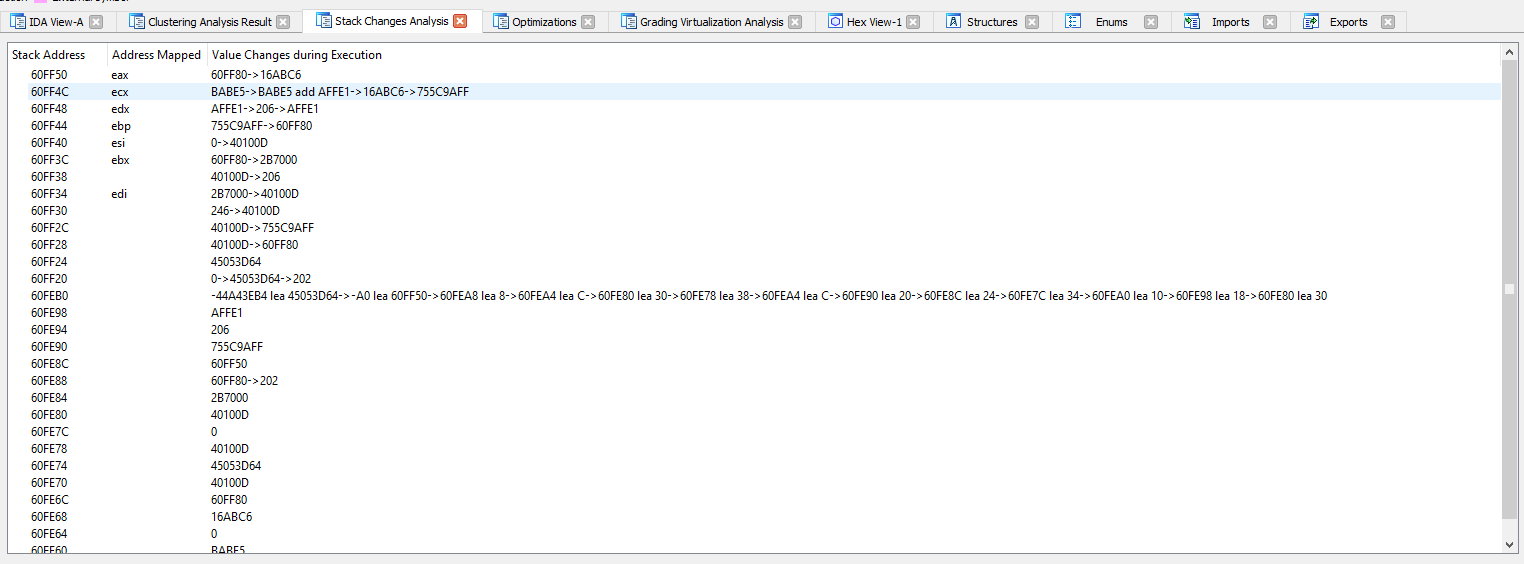
\includegraphics[scale=0.50]{images/ch3/StackChanges.png}
\caption{Abstract VM CFG created from the deobfuscated byte codes.}
\label{}
\end{figure}

\subsubsection{Grading Analysis View}
\todo{}
\begin{figure}[H]
\centering
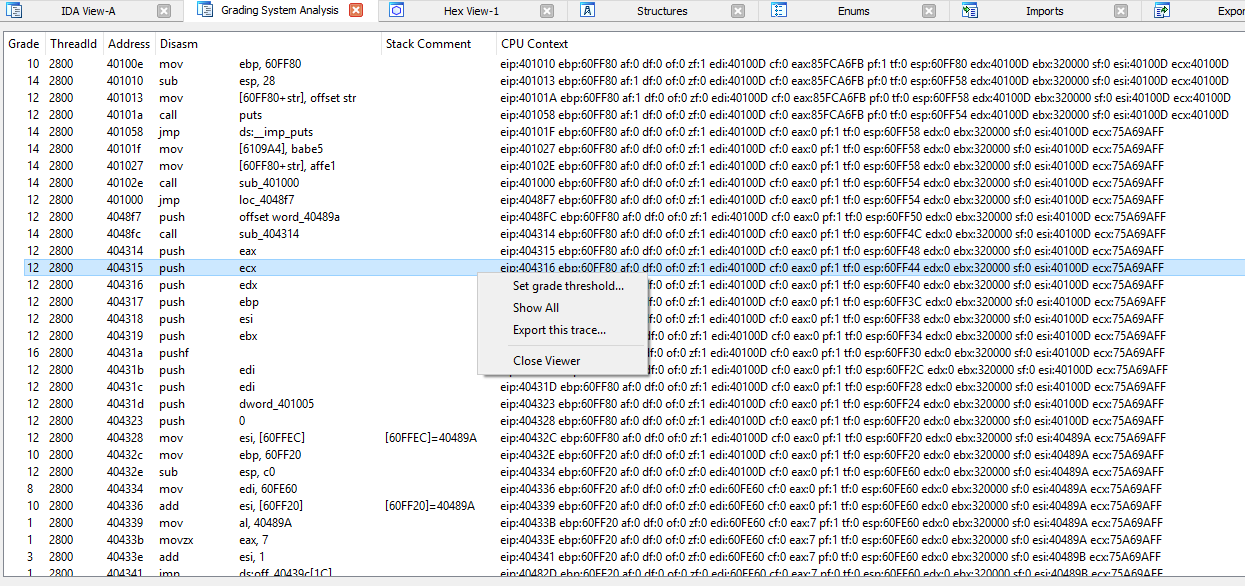
\includegraphics[scale=0.60]{images/ch3/grading1.png}
\caption{Abstract VM CFG created from the deobfuscated byte codes.}
\label{}
\end{figure}

\subsubsection{Static Abstract Control Flow Graph}
\todo{}
\begin{figure}[H]
\centering
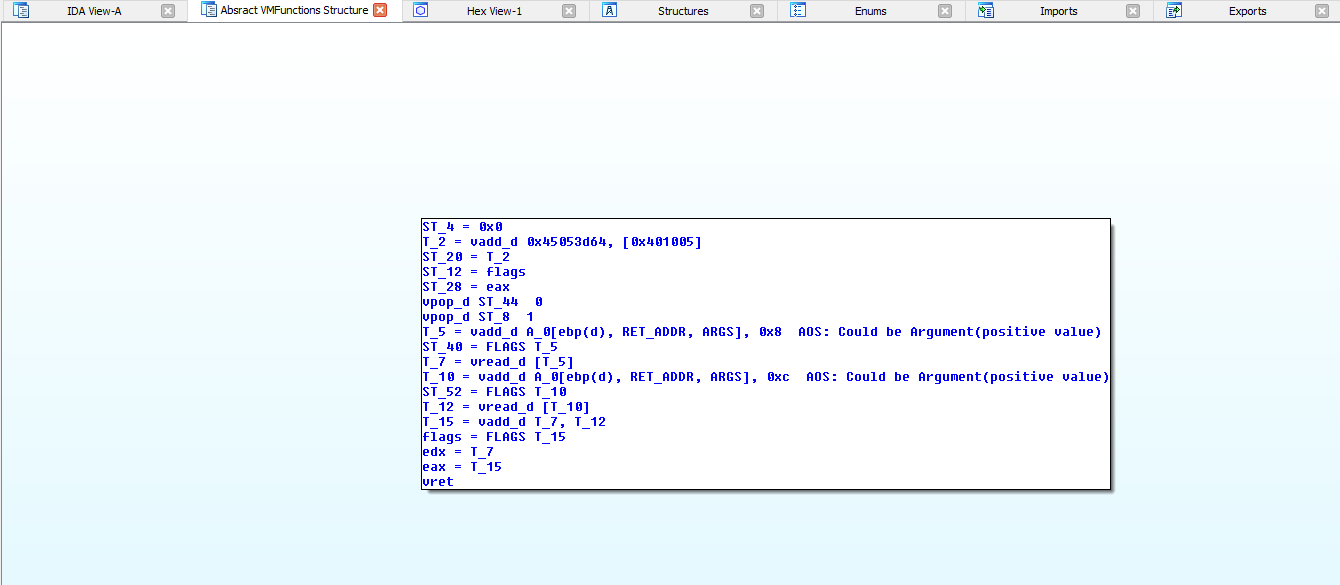
\includegraphics[scale=0.60]{images/ch3/ab_vm_graph.png}
\caption{Abstract VM CFG created from the deobfuscated byte codes.}
\label{}
\end{figure}


\section{Interaction with the Framework parameters}
\label{sec3:settings}
The Settings provide the necessary interface to enable the user to change values on the fly or even input own values if the ones determined by the plug-in are wrong. Further changes in the default behavior of the program can also be selected or removed.\\
The first section allows for configuration of the VM context. If the dynamic or static detection was already executed, the determined values are shown in their corresponding fields, if not -1 is shown. The user can simply override the current value by inputting another number. Thus, mistakes made in the parameter detection can easily be mitigated.\\
The next section deals with the clustering analysis. The 'Show basic blocks' option allows to disable the basic block summary and the differentiation of clusters into basic blocks in the clustering viewer. 
The second option allows for the deactivation of greedy clustering during the cluster analysis. Should greedy clustering be disabled, the user will be asked, how many rounds clustering shall proceed.
An important factor is the 'Cluster Heuristic'. 
This value determines how often values have to repeat to be considered a cluster. 
The default is two, which means, that an instruction has to be repeated at least two times to be considered a cluster.\\
The following section deals with the grading analysis. All available grading analysis components are listed here with an importance parameter. 
As this importance parameter changes, so does the weight an analysis has on the grading system. 
To disable an analysis completely set the according parameter to zero.\\
The last section covers the trace generation. It allows for enabling the 'Stepping into system Libraries' setting and to disable function parameter extraction, if the user does not wish to perform it. 


\begin{figure}[htp]
\centering
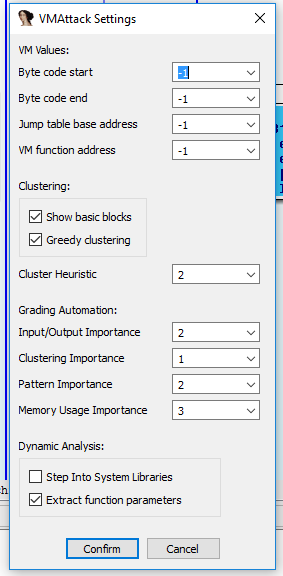
\includegraphics[scale=0.60]{images/ch3/settings.png}
\caption{Settings parameter overview.}
\label{settings}
\end{figure}

%%%%%%%%%%%%%%%%%%%%%%%%%%%%%%%%%%%%%%%%%%%%%%%%%%%%%%%%%%%%%%%%%%%%%%%%%%%%%%%
%
% Evaluation
% 
%%%%%%%%%%%%%%%%%%%%%%%%%%%%%%%%%%%%%%%%%%%%%%%%%%%%%%%%%%%%%%%%%%%%%%%%%%%%%%%


\chapter{Evaluation}
\label{sec4:evaluation}
\section{Evaluation structure}

This chapter handles the evaluation of the previously described framework, VMAttack. To represent different viewpoints and challenges to the analysis and deobfuscation methods ten simple programms were compiled, obfuscated with test version of VMProtect software and finally deobfuscated with VMAttack. Subject of evaluation is in the context of this thesis only the dynamic analysis capabilities and the 'grading system', which is the automated analysis. Execution of the binaries commenced on a x86 infrastructure in most cases but the results can be (and in fact were) easily reproduced on x64 architectures. As already explained in the Implementation\label{sec3:implementation} chapter, before the dynamic analysis can be enabled an instruction trace of the binary must either be generated or loaded from file. This step will not be mentioned every time as it is seen as a prerequisite for dynamic analysis.\\
As the output of the automatic analysis is graded with a high granularity and can always be dynamically adjusted by the user, it is necessary for the evaluation process to reflect these degrees of freedom accordingly. Therefore the grading system will be first tested with default parameters and only if the relevant instructions are not easily recognizable in the output the option of user defined weighting factors will be made use of. \\
The evaluation process for the dynamic analysis will judge the dynamic framework analysis functions whether the output can lead to the recovery of assembler instructions similar to those of the unobfuscated function. Two factors seem important in this context, on one hand the number of user interactions necessary for deobfuscation


\begin{center}
\begin{tabular}{l|l|l|l}
	\hline
	Binary function & Optimization & Input/Output & Clustering\\
	\hline
	add & 90 per cent & 90 per cent & 90 per cent\\
	mul & 90 per cent & 90 per cent & 90 per cent\\
	div & 90 per cent & 90 per cent & 90 per cent\\
	divd & 90 per cent & 90 per cent & 90 per cent\\
	sub & 90 per cent & 90 per cent & 90 per cent\\
	fibbonacci32 & 90 per cent & 90 per cent & 90 per cent\\
	fibbonacci64 & 90 per cent & 90 per cent & 90 per cent\\
	array & 90 per cent & 90 per cent & 90 per cent\\
	branch & 90 per cent & 90 per cent & 90 per cent\\
	\hline
\end{tabular}
\captionof{table}{The instruction trace reduction of different analysis techniques.}
\end{center}

\begin{center}
\begin{tabular}{l|l|l|l|l}
	\hline
	Binary function & Automatic analysis & Grading grade & Dynamic context & Static context\\
	\hline
	add & conclusively solved & best grade & 4 values correct & 4 values correct\\
	mul & conclusively solved & best grade & 4 values correct & 4 values correct\\
	div & conclusively solved & best grade & 4 values correct & 4 values correct\\
	divd & conclusively solved & best grade & 4 values correct & 4 values correct\\
	sub & conclusively solved & best grade & 4 values correct & 4 values correct\\
	fibbona32 & conclusively solved & best grade & 4 values correct & 4 values correct\\
	fibbona64 & conclusively solved & best grade & 4 values correct & 4 values correct\\
	array & conclusively solved & best grade & 4 values correct & 4 values correct\\
	branch & conclusively solved & best grade & 4 values correct & 4 values correct\\
	\hline
\end{tabular}
\end{center}



\section{Obfuscated add function}
The addvmp binary is basically a simple add function which takes two values, AFFE1 and BABE5, and adds them together, returning the result.
The Example folder contains the obfuscated binary and source binary of an add function. The obfuscated **addvmp** contains the VM function which we will analyze now.

\subsection{Automated analysis}
\subsection{Manual analysis}
\begin{figure}[htp]
\centering
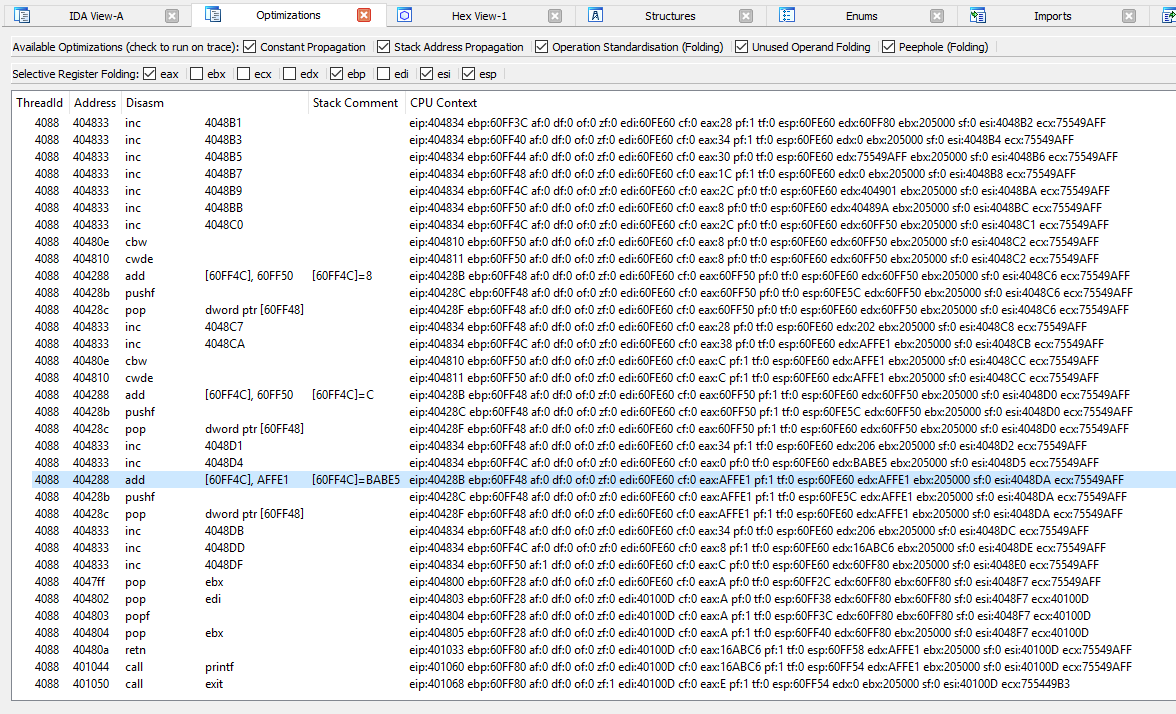
\includegraphics[scale=0.55]{images/ch3/optimizations_success.png}
\caption{Optimizations representation.}
\label{opti_add_success}
\end{figure}
![alt text](screenshots/overview.png "Problem Statement")

After a quick glance over the binary we see the simple structure: two arguments, `0AFFE1` and `0BABE5` are deployed on the stack and then a stub is called.
 
 \begin{figure}[htp]
\centering
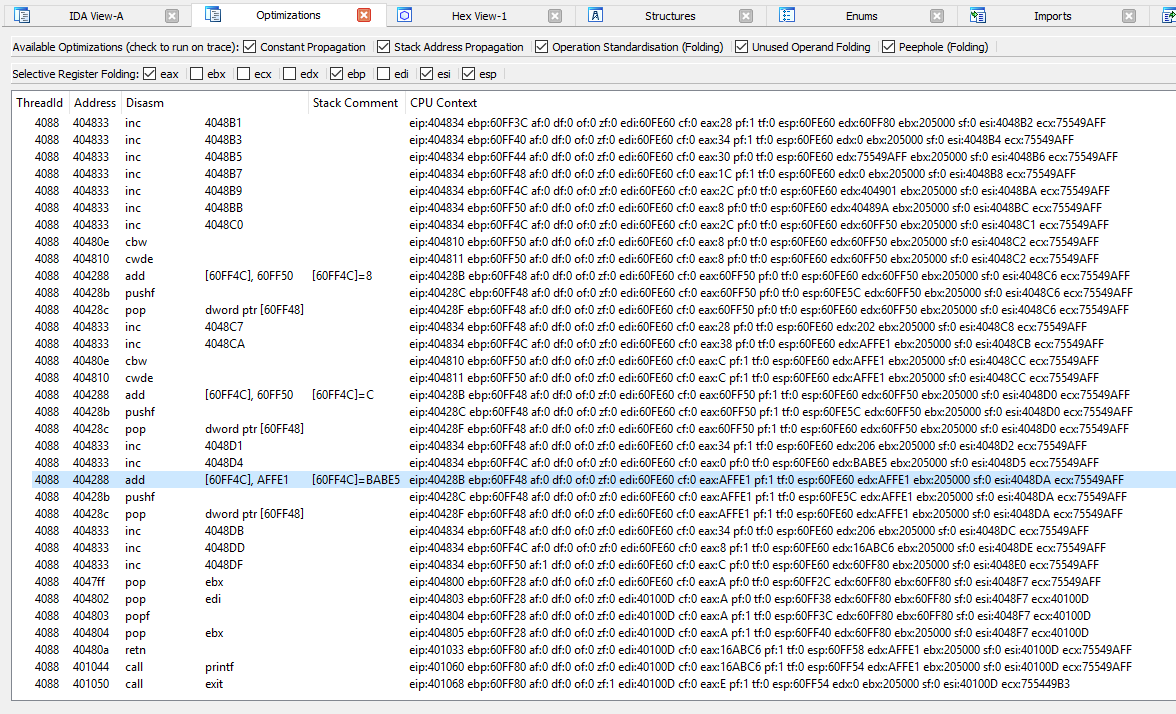
\includegraphics[scale=0.55]{images/ch3/optimizations_success.png}
\caption{Optimizations representation.}
\label{opti_add_success}
\end{figure}
![alt text](screenshots/stub.png "Problem Statement")
 
The stub starts the virtual machine function with a reference to the start of the VM byte code pushed onto the stack.

\begin{figure}[htp]
\centering
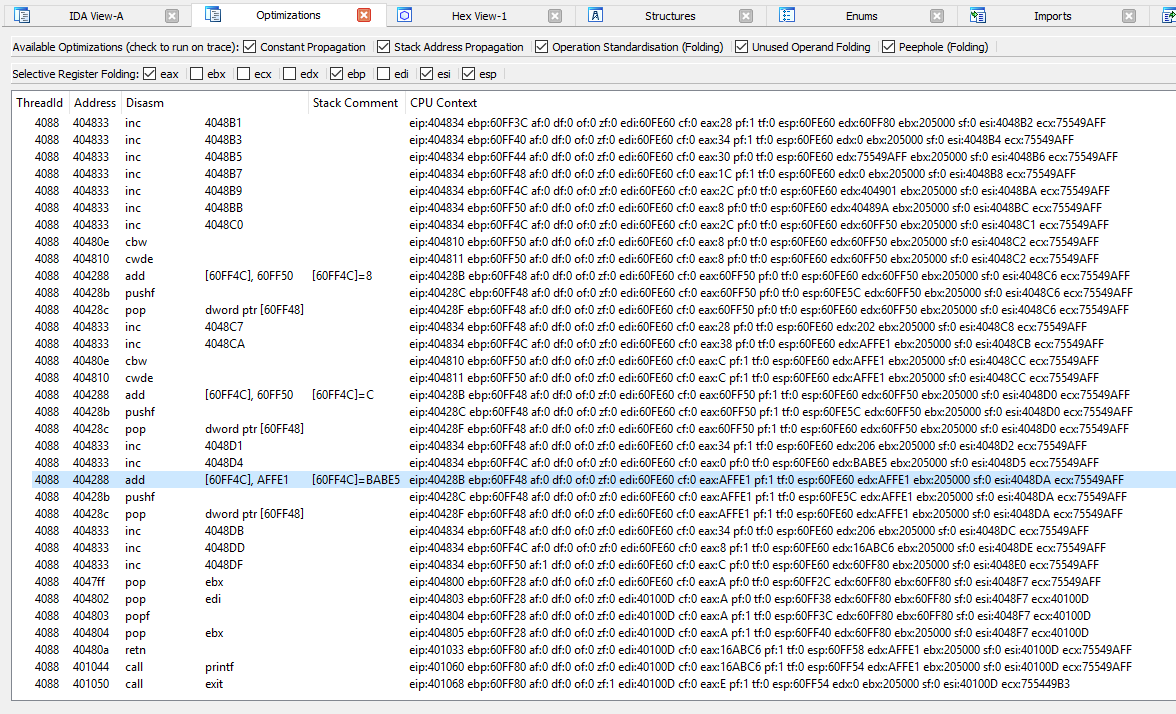
\includegraphics[scale=0.55]{images/ch3/optimizations_success.png}
\caption{Optimizations representation.}
\label{opti_add_success}
\end{figure}
![alt text](screenshots/stub2.png "Problem Statement")

Following the address we see the virtual machine function which is basically an interpreter for the received byte code.

\begin{figure}[htp]
\centering
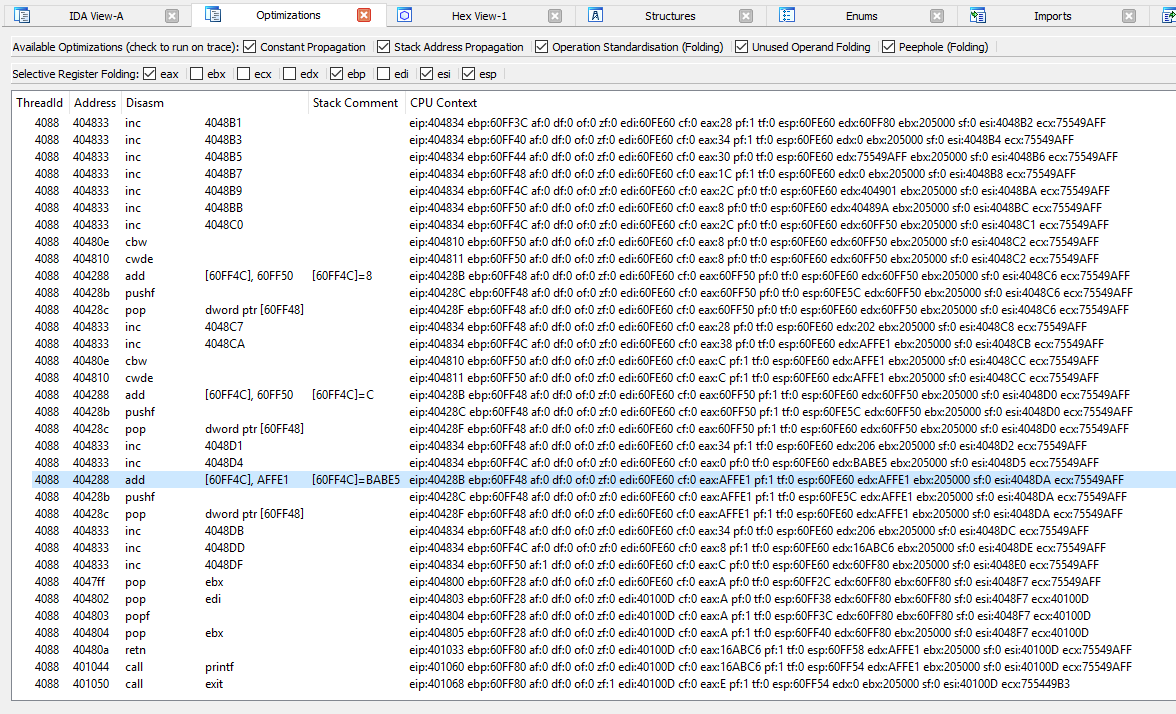
\includegraphics[scale=0.55]{images/ch3/optimizations_success.png}
\caption{Optimizations representation.}
\label{opti_add_success}
\end{figure}
![alt text](screenshots/switch.png "Interpreter")

A solution to this obfuscation would be the reversal of the interpreter and the interpretation of the byte code by the reverse engineer. Due to the time consuming nature of this task we will try to reverse the binary with our VMAttack plugin.

VMAttacks static analysis functionality is enabled by default. The dynamic analysis capabilities however require an extra step. Since we want to use the static and dynamic capabilities for this demo, first we need to enable the dynamic functionality of VMAttack. This is done by either generating an instruction trace dynamically or loading an instruction trace from file. Trace generation is automatic and upon completion it will produce a success notification in **IDA**s output window. Traversed paths will be colored in a shade of blue, where a darker shade represents a higher number of traversals. Alternatively the loaded trace will only produce the success notification in **IDA**s output window .
With the newly generated/loaded trace we now have dynamic an static capabilities enabled and can start the  grading system analysis . Starting with the  grading analysis  is usually a good fit, since it is automated and takes several analysis capabilities into account. This enables a **cumulative** result which can even tolerate analysis errors to some extent and still produce good results. At the end of the grading analysis the now graded trace will be presented in the **grading viewer**. The trace can now be filtered either by double clicking a grade or via context menu where the user will be prompted to input the grade threshold to display.
In the case of addvmp it will be enough to select the highest grade to be presented with the deobfuscated function (since the original function is quite simple in this case). In becomes obvious, that the two values passed over the stack are added together. Additionally, should the result be not satisfiable, the user can change the importance of an analysis function (**see settings**) or even disable them (by setting the importance to 0), to produce better results. Simply change the importance and re-run the grading analysis.

\begin{figure}[htp]
\centering
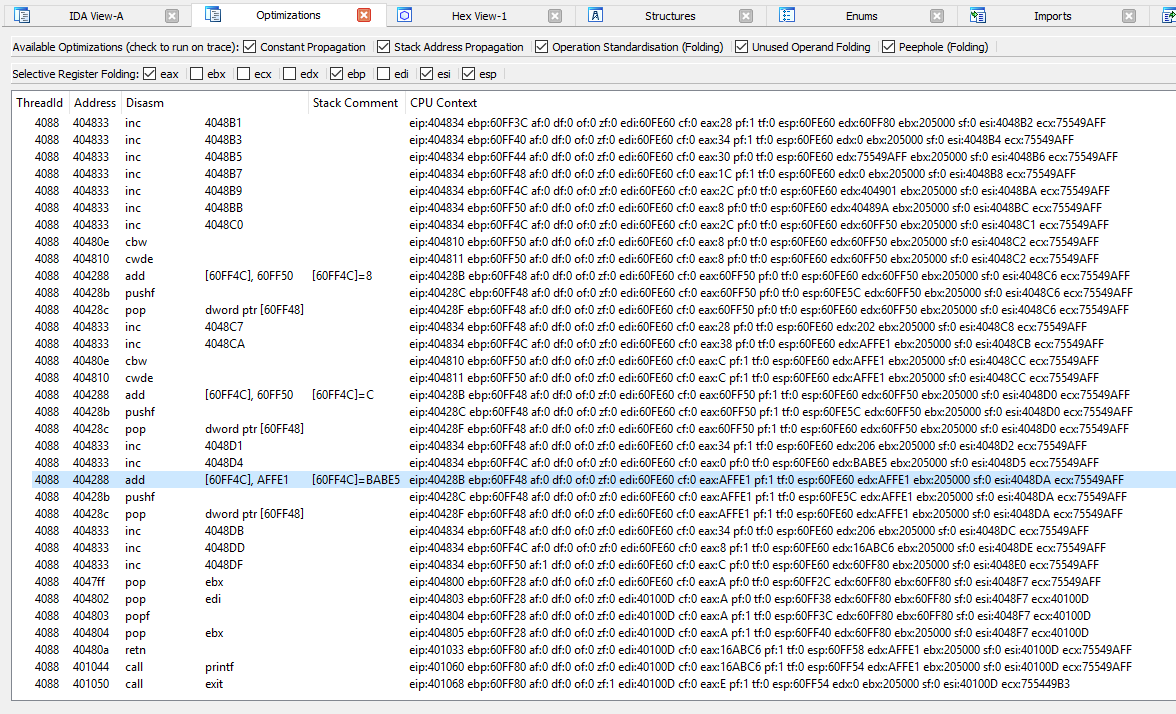
\includegraphics[scale=0.55]{images/ch3/optimizations_success.png}
\caption{Optimizations representation.}
\label{opti_add_success}
\end{figure}
![alt text](screenshots/grading4.png "Grading Success")

Lets assume we have a more complicated function and the  grading analysis  did not lead us to the relevant instructions.
One of the  semi-automated analysis  capabilities could present a viable alternative or even show us which analysis function failed the grading system.
The  input/output analysis  could provide leads as to how the input arguments of the VM function are used and whether there is a connection between function input and function output. By checking the two input values `AFFE1` and `BABE5` and additionally the output value `16ABC6` it becomes evident which register contains the important instructions for out obfuscated function and how the `eax` return value came to be `16ABC6`.


\begin{figure}[htp]
\centering
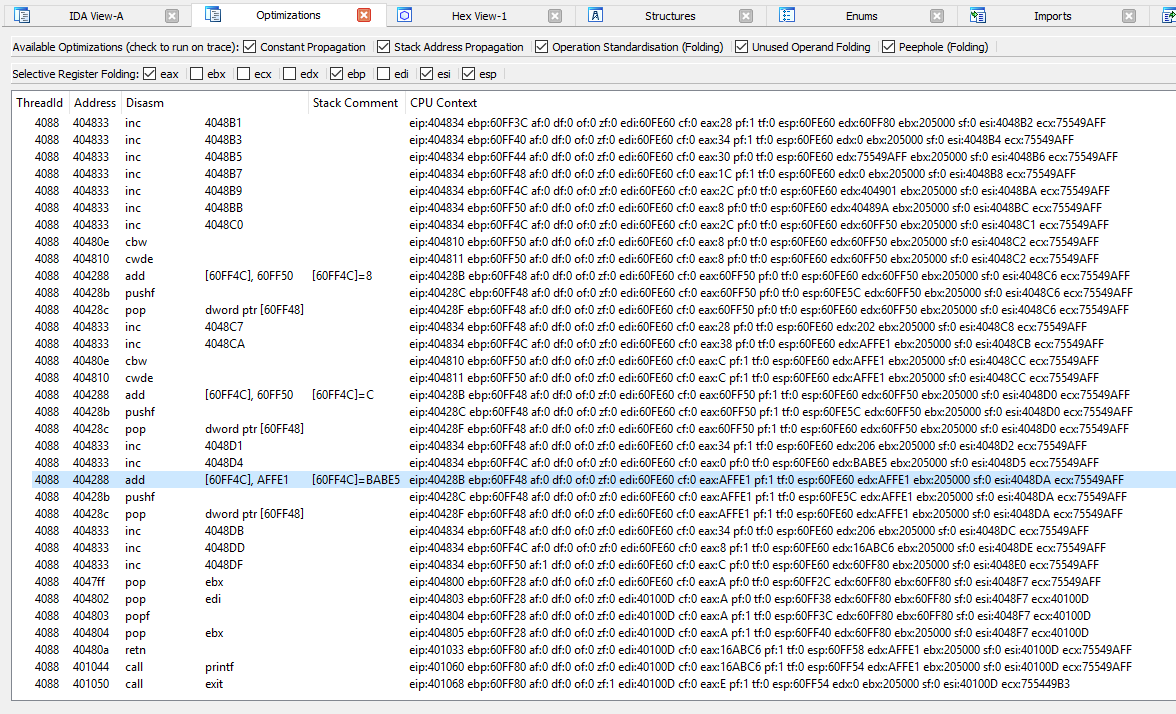
\includegraphics[scale=0.55]{images/ch3/optimizations_success.png}
\caption{Optimizations representation.}
\label{opti_add_success}
\end{figure}
![alt text](screenshots/InputOutput3.png "Input/Output Success")

Another powerful functionality is the  clustering analysis . It enables the reverse engineer to quickly discern between repeating instructions and unique ones. The  clustering analysis view  additionally enables quick removal of unnecessary clusters (or instructions) in a way speeding up the work of the reverse engineer. Should a mistake be made it can be undone or alternatively the original trace can be restored. To make sense of the clustering analysis usually requires an extensive analysis of the trace and can require repeating the clustering analysis with a different cluster heuristic value set via **settings**.


\begin{figure}[htp]
\centering
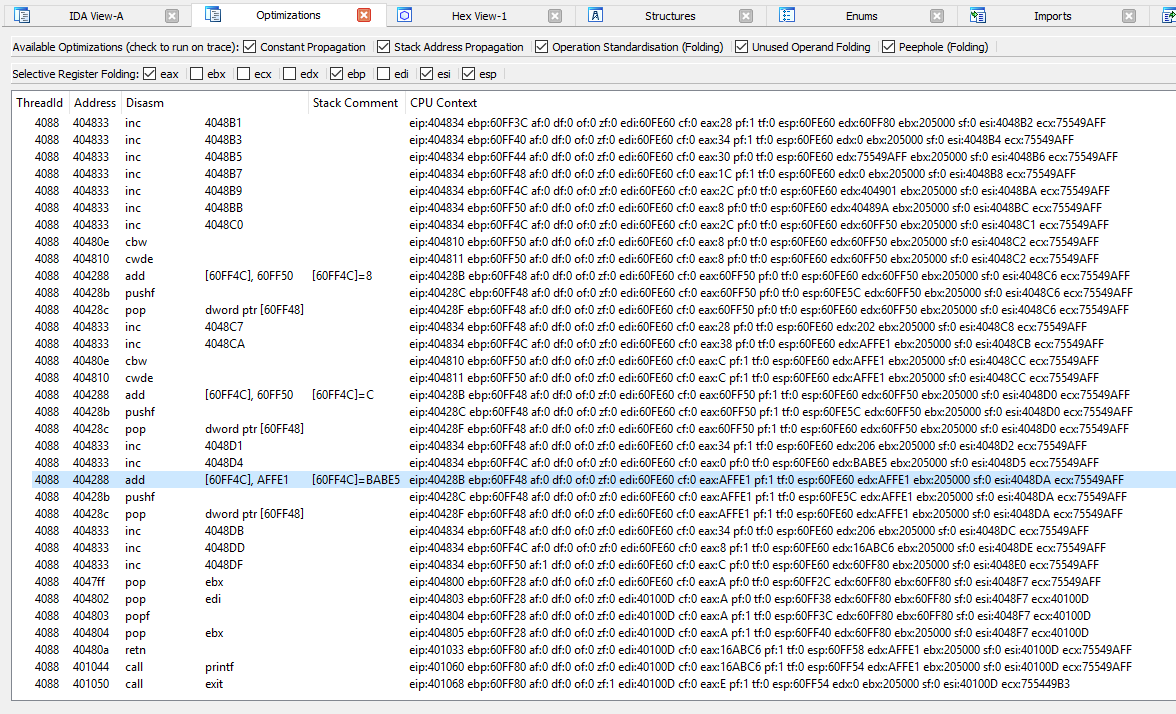
\includegraphics[scale=0.55]{images/ch3/optimizations_success.png}
\caption{Optimizations representation.}
\label{opti_add_success}
\end{figure}
![alt text](screenshots/clustering1.png "Input/Output Viewer")

Out of the semi-automatic analysis the  optimization analysis  requires the most user interaction. In turn it enables:

- Optimizations which make the trace easier to read or even filter as unnecessary recognized instructions. 
- Filtering capabilities to remove as unnecessary recognized instructions or even whole registers from the trace.
- Undoing actions if you made a mistake.
- Restoring the initial trace if you hit a wall.

\begin{figure}[htp]
\centering
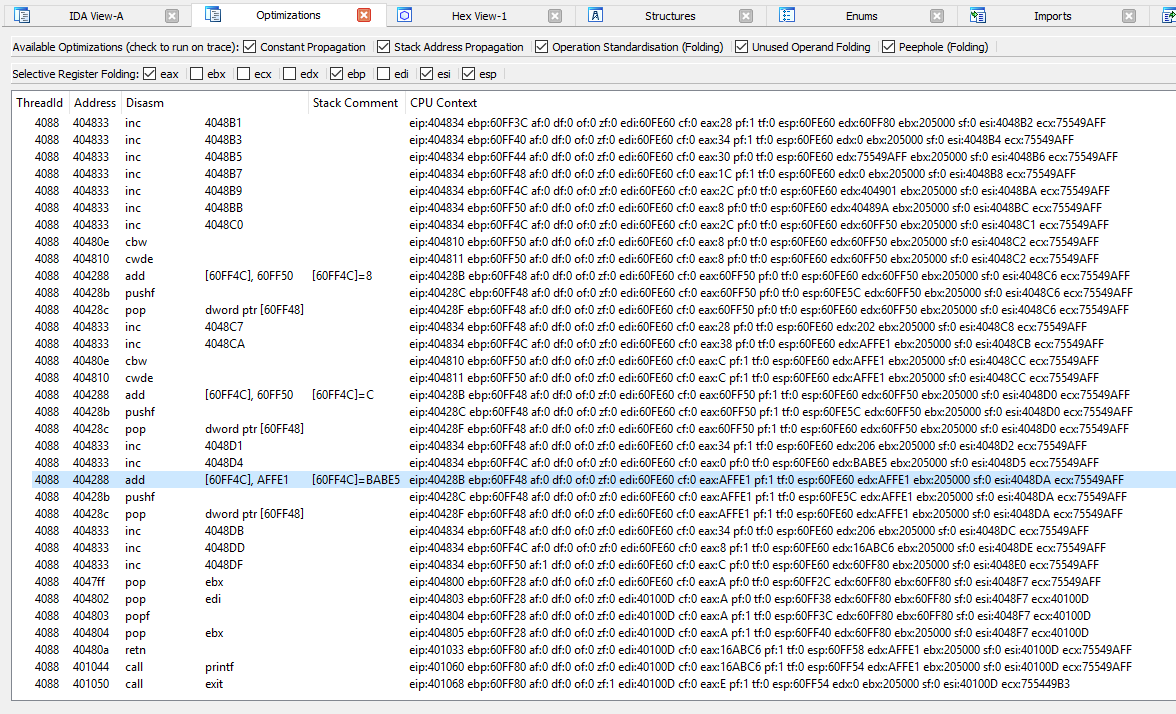
\includegraphics[scale=0.55]{images/ch3/optimizations_success.png}
\caption{Optimizations representation.}
\label{opti_add_success}
\end{figure}

The  static analysis  in this case would enable us to analyze the byte code and optionally view the analysis as an  abstract VM graph  of the byte code. The static deobfuscation of the byte code will produce comments behind relevant bytes to describe the operation this byte produces. The commented instructions are quite intuitive and should be easy to read.
The abstract VM graph in turn will produce a control flow graph (in the case of addvmp just one basic block) filled with those abstract instructions from the byte code. This is also a good example of the accuracy of the static analysis, which without execution delivered an accurate representation of the initial deobfuscated function. After the static analysis we can clearly see that two arguments were passed to the function  (AOS = acces out of known space; indicates for example arguments passed via stack)  and that they were eventually added together and then returned.

\begin{figure}[htp]
\centering
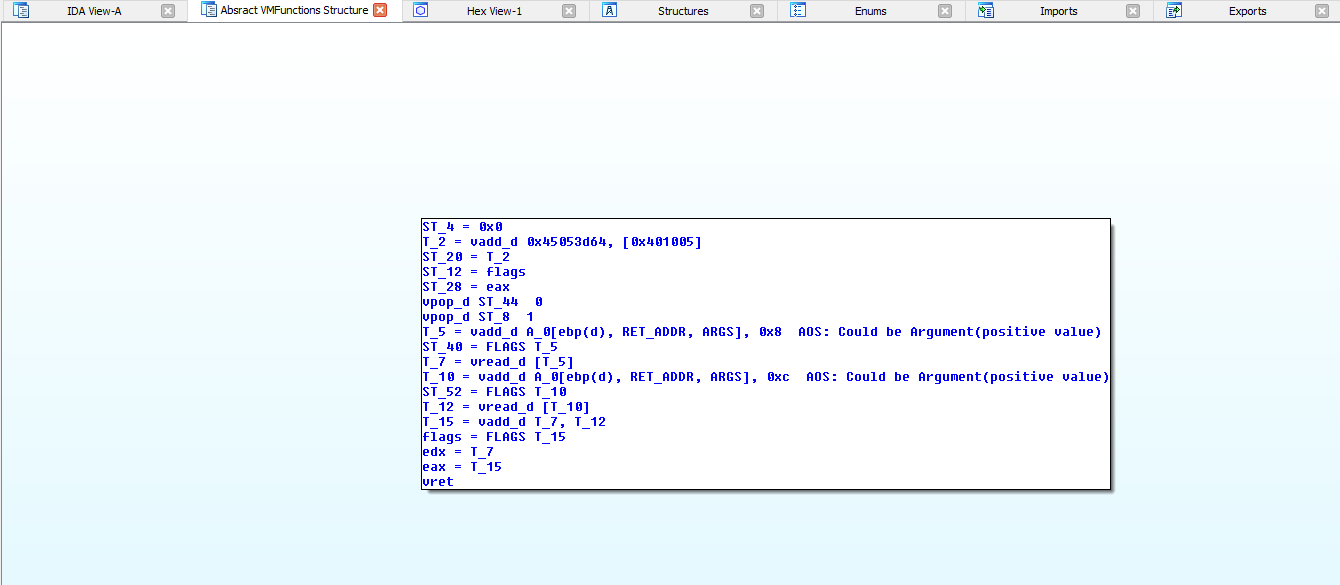
\includegraphics[scale=0.45]{images/ch3/ab_vm_graph.png}
\caption{Abstract VM graph representation.}
\label{abs_vm_graph}
\end{figure}

\section{Obfuscated mul function}
\subsection{Automated analysis}
\subsection{Manual analysis}
\section{Obfuscated div function}
\subsection{Automated analysis}
\subsection{Manual analysis}
\section{Obfuscated divd function}
\subsection{Automated analysis}
\subsection{Manual analysis}
\section{Obfuscated sub function}
\subsection{Automated analysis}
\subsection{Manual analysis}
\section{Obfuscated fibonacci functions}
\subsection{Automated analysis}
\subsection{Manual analysis}
\section{Obfuscated array function}
\subsection{Automated analysis}
\subsection{Manual analysis}
\section{Obfuscated branch function}
\subsection{Automated analysis}
\subsection{Manual analysis}

\fancyhead[RE]{\leftmark}
%%%%%%%%%%%%%%%%%%%%%%%%%%%%%%%%%%%%%%%%%%%%%%%%%%%%%%%%%%%%%%%%%%%%%%%%%%%%%%%
%
% Conclusion and Future Work
% 
%%%%%%%%%%%%%%%%%%%%%%%%%%%%%%%%%%%%%%%%%%%%%%%%%%%%%%%%%%%%%%%%%%%%%%%%%%%%%%%


\chapter{Conclusion and Future Work}
\label{sec5:conclusion_and_future_work}


\section{Future Work}
\subsection{Code Coverage}

\subsection{Additional Optimization Techniques}

\subsection{Additional Analysis Techniques}

\subsection{Additional Obfuscation Resistance}

\section{Conclusion}
This thesis describes a dynamic oriented framework, VMAttack, with several approaches at deobfuscation of virtualization obfuscated binaries which are combinable in a modular, automatable system. 
VMAttack provides an interactive, completely configurable approach and supports a wide array of versatile strategies for analysis. The capabilities primarily aim at stack based virtual machines but some also support other architectures. \\
The framework builds upon a previously developed static approach at virtualization deobfuscation. This static approach allows for deobfuscation of the virtual machine byte code without prior execution of the binary. It uses an easy to read intermediate representation to convey the meaning of every byte.
The newly introduced dynamic approach features powerful optimization techniques to enrich information available to the reverse engineer and dynamic analysis techniques than allow for extraction of relevant instructions of an execution trace. 
The key techniques are the Input/Output analysis, which backtraces the output values and deobfuscates the virtualization layer by establishing a connection between the VMs input and output parameters, and the Clustering analysis which enables the grouping of repeating instruction to classify unique functionality within the binary. \\
The robust automation system incorporates all available analysis techniques, static and dynamic, to provide a fault tolerant analysis result as a combination of these available analysis techniques. 
The combination of these techniques and their weight in the overall analysis can be controlled as needed and the result presentation can be interacted with dynamically to provide the best possible result.\\
Experiments with the free version of the commercial tool VMProtect suggest, that our approach is indeed effective and provides a highly aqurate analysis result and great improvements in terms of time needed for analysis and recovery of the deobfuscated original code.
The idea was met with approval from the reversing community, even winning first place in the IDA Plug-in Contest 2016.


\fancyhead[RE]{\rightmark}


% Bibliography
\bibliographystyle{plainnat}
\bibliography{thesis}

\cleardoublepage

%%%%%%%%%%%%%%%%%%%%%%%%%%%%%%%%%%%%%%%%%%%%%%%%%%%%%%%%%%%%%%%%%%%%%%%%%%%%%%%
%
% Appendix
% 
%%%%%%%%%%%%%%%%%%%%%%%%%%%%%%%%%%%%%%%%%%%%%%%%%%%%%%%%%%%%%%%%%%%%%%%%%%%%%%%
\begin{appendix}
\chapter{Appendix A $-$ New VMAttack Features}
\section{Installation}
\section{User Interface}
\section{Dynamic Analysis}
\section{Lib}

\end{appendix}


\end{document}
